% Capíulo 3
\chapter{Estudo sobre a Compatibilidade a Múltiplas Versões da API Android}
\label{ch:estudo}

Este capítulo apresenta o estudo realizado para análise do suporte de aplicações
existentes à múltiplas versões da API da plataforma Android. Foram analisados o
código-fonte de 41 aplicações únicas com o objetivo de identificar e caracterizar
as técnicas de implementação de variabilidades.

O restante do capítulo está organizado da seguinte maneira: 
a seção \ref{sec:objetivos} destaca os objetivos do estudo e as questões de pesquisa.
A seção \ref{sec:aplicacoes-alvo} apresenta os critérios de seleção das aplicações
alvo do estudo, bem como as aplicações selecionadas.
A seção \ref{sec:procedimentos} descreve os procedimentos adotados para responder
cada questão de pesquisa. 
A seção \ref{sec:resultados} apresenta os resultados do estudo, que são discutidos na
seção \ref{sec:discussao}.
Por fim, as ameaças à validade são reportadas na seção \ref{sec:ameacas}.

\section{Objetivos do Estudo e Questões de Pesquisa} \label{sec:objetivos}

Nosso estudo foi realizado com o objetivo de caracterizar, entender e analisar
como as aplicações Android lidam com múltiplas versões da API da plataforma, além
do impacto deste suporte no código-fonte das aplicações. Para atingir este objetivo,
o estudo foi guiado pelas seguintes questões de pesquisa (QPs):

\begin{itemize}
	\item \textbf{QP1}: Quais são as técnicas que aplicações atuais usam para manter
	compatibilidades com as diversas versões da API do Android? O objetivo dessa questão
	é indicar quais as técnicas vem sendo utilizadas e suas características, auxiliando
	desenvolvedores a decidirem o que e quando utilizar em suas aplicações.
		\begin{itemize}
			\item Essa questão foi respondida analisando no código-fonte das aplicações o
			uso de técnicas como: (i) pacotes de compatibilidade, (ii) re-implementação de
			recursos e (iii) acesso explícito às novas API's. Para este último caso,
			aprofundamos a análise para determinar como as aplicações evitam que chamadas
			a novas API's sejam feitas de forma indevida, o que causará uma interrupção na
			execução da aplicação.
		\end{itemize}
	\item \textbf{QP2}: Qual o subconjunto de novas funcionalidades da plataforma que são
	mais utilizadas por aplicações compatíveis com versões antigas da API? Esse levantamento
	auxilia desenvolvedores de aplicações Android a identificar os elementos que eles podem
	utilizar em suas aplicações, permitindo a concentração de esforços nesses elementos.
		\begin{itemize}
			\item Para responder essa questão, contabilizamos os elementos de API's utilizados
			pela aplicação e que são superiores a versão mínima especificado pela mesma. Seja
			através dos pacotes de compatibilidade, da re-implementação de recursos ou do acesso
			explícito às novas API's. Esse elementos foram agrupados pela taxonomia apresentada
			na seção \ref{sec:taxonomia}.
		\end{itemize}
	\item \textbf{QP3}:Qual o esforço necessário para aumentar a compatibilidade com um maior
	número de API's de versões anteriores da plataforma? Estabelecer uma versão elevada de API
	para execução do aplicativo pode significar deixar de atender um grande mercado potencial.
	Assim, a resposta para essa questão dará aos desenvolvedores um indicativo estimado do trabalho
	que terão para aumentar seu mercado potencial.
		\begin{itemize}
			\item Para responder essa questão, modificamos a versão mínima da API e verificamos quais
			novas ocorrências de NewApi são apresentadas pelo Android Lint, de forma a entender o
			esforço em termos de mudanças de código fonte para atender a mesma.
		\end{itemize}
	\item \textbf{QP4}: Qual a incidência de código morto em função da versão da API do Android? 
	A evolução da API mínima exigida pelas aplicações, aqui no sentido de edição da configuração
	no arquivo de manifesto, associada à execução condicional pode resultar em código-morto.
	Analisamos as aplicações para determinar se isso tem ocorrido com frequência e em qual volume.
		\begin{itemize}
			\item Essa questão foi respondida a partir da edição do código-fonte das aplicações.
			Localizamos e removemos todo o código relacionado à qualquer API inferior à mínima
			exigida pela aplicação.
		\end{itemize}
\end{itemize}

\section{Aplicações Alvo de estudo} \label{sec:aplicacoes-alvo}

As aplicações utilizados no estudo são aplicações \textit{open-source} populares,
com um mínimo de 6 mil linhas de código, contabilizados arquivos Java e XML, e de
categorias diversas. Um das aplicações possui 10 mil downloads na Google Play,
outra possui 50 mil \textit{downloads} e as demais mais de 100 mil.

Analisamos um total de 41 aplicações únicas. Não analisamos todas as aplicações em
todas as questões, mas algumas aplicações foram analisadas em mais de uma questão.
Isso ocorreu devido a natureza das nossas questões de pesquisa, que exigiu a análise
de grupos diferentes de aplicações para determinadas questões, com critérios de seleção
adicionais aos citados anteriormente. Assim, definimos 3 grupos de aplicações, apresentados
a seguir.

\subsection{Grupo 1 - Aplicações usando API da plataforma com grande variação de versões}
Aplicações do grupo 1 possuem uma diferença de pelo menos 7 versões entre a API mínima e
a API alvo. A nossa hipótese é que além da aplicação oferecer suporte para versões de API's
antigas também utiliza recursos das versões mais recentes da API quando disponíveis. Tais
aplicações foram utilizadas para responder às questões QP1 e QP2 e são listadas na tabela
\ref{tab:grupo1}. São 25 aplicações nesse grupo.

\begin{table}[!htbp] % TODO posicionar melhor essa tabela
  \centering
  \caption{Aplicações usando API da plataforma com grande variação de versões}
  \begin{tabular}{| l | l | r | r | r | r |}
  	\hline
  	% rótulo das columnas
  	\multicolumn{1}{|c|}{\textbf{Aplicação}} &
  	\multicolumn{1}{c|}{\textbf{Categoria}} &
 	\multicolumn{1}{c|}{\textbf{Downloads}} & 
 	\begin{tabular}[c]{@{}c@{}}
 		\textbf{API}\\ \textbf{Mínima}
 	\end{tabular} &
 	\begin{tabular}[c]{@{}c@{}}\textbf{API}\\ \textbf{Alvo}\end{tabular} &
 	\multicolumn{1}{c|}{\textbf{KLoc}} \\ \hline
 	%dados
 	Wififixer 		& Ferramentas 			& 1.000.000   &  7 & 23 &   9 \\ \hline
 	AnySoftKeyBoard & Ferramentas 			& 1.000.000   &  7 & 23 & 180 \\ \hline
 	Telegram 		& Comunicação 			& 100.000.000 &  9 & 23 & 169 \\ \hline
 	AntennaPod  	& Mídia e Video 		& 100.000 	  & 10 & 23 &  65 \\ \hline
 	Google I/O   	& Livros e Referências 	& 500.000 	  & 14 & 22 &  52 \\ \hline
 	Firefox    		& Comunicação 			& 100.000.000 & 15 & 22 & 233 \\ \hline
 	AnkiDroid     	& Educação 				& 1.000.000   & 10 & 22 &  89 \\ \hline
 	K-9 Mail      	& Comunicação 			& 5.000.000   & 15 & 22 & 117 \\ \hline
 	C:Geo       	& Entretenimento 		& 1.000.000   &  9 & 21 & 123 \\ \hline
 	Zmanim        	& Estilo de Vida 		& 10.000 	  & 10 & 22 &  25  \\ \hline
 	\begin{tabular}[l]{@{}l@{}}
 		Simon Tatham's \\ Puzzles
 	\end{tabular} 	& Quebra-cabeças 		& 100.000 	  &  7 & 23 &   8  \\ \hline
 	Vuze Remote     & Ferramentas			& 100.000	  &  7 & 23 &  20 \\ \hline
 	VLC for Android & 
 	\begin{tabular}[l]{@{}l@{}} Reproduzir e \\
 	 		 editar vídeos \end{tabular}    & 50.000.000  &  8 & 23 &  65 \\ \hline
 	\begin{tabular}[l]{@{}l@{}}
 	 	DuckDuckGo \\ Search \& Stories
 	\end{tabular}   & Livros e referências  & 1.000.000   &  8 & 23 &  23 \\ \hline
 	\begin{tabular}[l]{@{}l@{}}
 		Shattered Pixel \\ Dungeon
 	\end{tabular} 	& RPG 					& 500.000     &  8 & 23 &  58 \\ \hline
 	Persian Calendar& Produtividade			& 100.000 	  &  8 & 23 &  10 \\ \hline
 	Free Mobile Netstat& Ferramentas  		& 100.000 	  &  8 & 23 &   6 \\ \hline
 	MyExpenses    & Finanças 			& 100.000     &  8 & 23 &  80 \\ \hline
    \begin{tabular}[l]{@{}l@{}}
    	Simple Last.fm \\ Scrobbler
    \end{tabular} 	   & Música e áudio     & 500.000     &  7 & 22 &  10 \\ \hline
    Document Viewer	   & Produtividade		& 500.000 	  &  8 & 22 &  77 \\ \hline
	OpenTasks		   & Produtividade      & 100.000     &  8 & 22 &  23 \\ \hline
	\begin{tabular}[l]{@{}l@{}}
		Terminal Emulator \\ for Android
	\end{tabular} 	   & Ferramentas		& 10.000.000  &  4 & 22 &  18 \\ \hline
	ConnectBot		   & Comunicação	    & 1.000.000   &  4 & 22 &  24 \\ \hline
	Quick Dice Roller  & Ferramentas		& 100.000 	  &  4 & 21 &  35 \\ \hline
	\begin{tabular}[l]{@{}l@{}}
		BatteryBot Battery \\ Indicator
	\end{tabular} 	   & Ferramentas		& 5.000.000   &  7 & 22 &  6 \\ \hline
  \end{tabular}
  \label{tab:grupo1}
\end{table}

\subsection{Grupo 2 - Aplicações usando apenas API's mais recentes}
Aplicações do grupo 2 possuem um alto valor de API mínima mas não tem um histórico de suporte
às versões anteriores. Para esse estudo, as versões iguais ou superiores à 16 foram consideradas
como alta. Versões inferiores a esta representam 3.4\% do mercado mundial, conforme pode ser visto
na figura \ref{fig:platform_versions}. E para caracterizar ausência de um histórico de suporte
às versões anteriores,
consideramos aquelas cuja API mínima inicial seja igual ou superior a 11. A nossa hipótese é que
a aplicação foi criada sem a preocupação de oferecer suporte às versões antigas da API o que,
possivelmente, a leva a perder uma fatia do mercado de aplicações. Tais aplicações foram utilizadas
para responder à questão QP3 e estão listadas na tabela \ref{tab:grupo2}. São 10 aplicações nesse grupo.

\begin{table}[!htbp]
  \centering
  \caption{Aplicações usando apenas API's mais recentes}
  \begin{tabular}{| l | l | r | r | r | r |}
  	\hline
  	% rótulo das columnas
  	\multicolumn{1}{|c|}{\textbf{Aplicação}} &
  	\multicolumn{1}{c|}{\textbf{Categoria}} &
 	\multicolumn{1}{c|}{\textbf{Downloads}} & 
 	\begin{tabular}[c]{@{}c@{}}
 		\textbf{API}\\ \textbf{Mínima} \\ \textbf{Inicial}
 	\end{tabular} &
 	\begin{tabular}[c]{@{}c@{}}\textbf{API}\\ \textbf{Mínima}\\ \textbf{Atual}\end{tabular} &
 	\multicolumn{1}{c|}{\textbf{KLoc}} \\ \hline
 	% dados
 	AcDisplay 		& Personalização 		& 1.000.000   & 19 & 16 & 40 \\ \hline
 	Dash Clock		& Personalização		& 1.000.000   & 17 & 17 & 15 \\ \hline
 	Focal (Beta) 	& Fotografia 			& 500.000	  & 16 & 16 &  16 \\ \hline
 	\begin{tabular}[l]{@{}l@{}}
 	 		Hangar - Smart \\ app shortcuts
 	\end{tabular}	& Ferramentas 		& 50.000 	  & 16 & 16 &  12 \\ \hline
 	Indic Keyboard  & Ferramentas 	& 100.000 	  & 14 & 16 &  81 \\ \hline
 	\begin{tabular}[l]{@{}l@{}}
 	 	 	Numix Circle \\ icon pack
 	\end{tabular}   & Personalização    	& 100.000 	  & 11 & 16 &   8 \\ \hline
 	SnoopSnitch     & Ferramentas 			& 100.000     & 14 & 16 &  17 \\ \hline
 	Termux      	& Ferramentas 			& 100.000	  & 21 & 21 &  10 \\ \hline
 	\begin{tabular}[l]{@{}l@{}}
 	 		WiFiAnalyzer \\ (open-source)
 	\end{tabular}   & Ferramentas 			& 100.000     & 22 & 21 &  12 \\ \hline
 	\begin{tabular}[l]{@{}l@{}}
 		Yaac - \\ IRC Client
 	\end{tabular} 	& Ferramentas 			& 50.000 	  & 16 & 16 &  12  \\ \hline
 	\end{tabular}
  \label{tab:grupo2}
\end{table}


\subsection{Grupo 3 - Aplicações usando API's recentes com histórico de uso de API's antigas}
Aplicações do grupo 3 possuem um alto valor de API mínima e também um histórico
de suporte às versões anteriores. Para esse grupo de aplicações, consideramos
aquelas cuja versão da API seja igual ou superior a 15 e a API mínima inicia
menor ou igual a 8. Nossa hipótese é que as aplicações possuem código-morto,
que só seriam executados na presença de API's antigas. Tais aplicações foram
utilizadas para responder à questão QP4 e estão listadas na tabela \ref{tab:grupo3}.
São 7 aplicações nesse grupo.

\begin{table}[!htbp]
  \centering
  \caption{Aplicações usando API's recentes com histórico de uso de API's antigas}
  \begin{tabular}{| l | l | r | r | r | r |}
  	\hline
  	% rótulo das columnas
  	\multicolumn{1}{|c|}{\textbf{Aplicação}} &
  	\multicolumn{1}{c|}{\textbf{Categoria}} &
 	\multicolumn{1}{c|}{\textbf{Downloads}} & 
 	\begin{tabular}[c]{@{}c@{}}
 		\textbf{API}\\ \textbf{Mínima} \\ \textbf{Inicial}
 	\end{tabular} &
 	\begin{tabular}[c]{@{}c@{}}\textbf{API}\\ \textbf{Mínima}\\ \textbf{Atual}\end{tabular} &
 	\multicolumn{1}{c|}{\textbf{KLoc}} \\ \hline
 	% dados
 	AFWall+ 		& Ferramentas	 		& 500.000     & 7  & 15 & 32 \\ \hline
 	aMetro			& 
 	\begin{tabular}[l]{@{}l@{}}
 	 	Mapas e \\ Navegação \end{tabular}	& 100.000	  & 3 & 15 &  10 \\ \hline
 	\begin{tabular}[l]{@{}l@{}}
 	 		Hangar - Smart \\ app shortcuts
 	\end{tabular}	& Ferramentas 		& 50.000 	  & 16 & 16 &   12 \\ \hline
 	K-9 Mail  		& Comunicação 		& 5.000.000	  &  3 & 15 &  117 \\ \hline
 	\begin{tabular}[l]{@{}l@{}}
 	 	 	Orbot Proxy \\ com Tor
 	\end{tabular}   & Comunicação    	& 5.000.000 	  & 4 & 16 & 33 \\ \hline
 	Ringdroid     	&
 	\begin{tabular}[l]{@{}l@{}} Reproduzir e \\
 	 	 	Editar Vídeos \end{tabular}	& 50.000.000	  & 4 & 16 &   6 \\ \hline
 	Transdrone      & Ferramentas 		& 100.000	      & 4 & 15 &  36 \\ \hline
 	\begin{tabular}[l]{@{}l@{}}
 	 		Vanilla Music
 	\end{tabular}   & Música e Áudio 			& 500.000     &  3 & 15 & 25 \\ \hline
 	\end{tabular}
  \label{tab:grupo3}
\end{table}

\section{Procedimentos} \label{sec:procedimentos}

Uma vez selecionadas as aplicações alvos do estudo, foi realizada a atividade de
análise das aplicações para buscar respostas às questões de pesquisa. A seguir,
descrevemos os procedimentos adotados. 

\subsection{Questões QP1 e QP2}
Para responder às questões de pesquisa QP1 e QP2, os procedimentos adotados foram os
seguintes:

\begin{enumerate}
	\item Remoção das anotações \texttt{@TargetAPI}, \texttt{@SuppressWarnings},
	 	\texttt{@SuppressLint} do código-fonte da aplicação. Essas remoções foram
	 	 necessárias porque tais anotações servem para silenciar o Lint, omitindo 
	 	 ocorrências do relatório; 
	\item Execução do Android Lint na aplicação;
	\item Para cada ocorrência de NewAPI, o contexto era analisado de forma manual
		para determinar se:
		\begin{itemize}
			\item Trata-se da implementação do padrão Execução Condicional
				\cite{Santos2012};
			\item Implementação é baseada em padrões de projeto \cite{Gamma}; 
			\item Ou algum outro mecanismo que evitasse a chamada em uma versão
			da API cujo recurso está ausente;
		\end{itemize}
	\item Para cada ocorrência de NewAPI, de forma semiautomática, o elemento da API
		era classificado de acordo com a taxonomia apresentada na seção \ref{sec:taxonomia};
	\item Nos aplicativos que utilizam pacote de compatibilidade, os elementos foram
		 classificados na taxonomia com uma busca pelos \texttt{import}'s  presentes
		 nas classes das aplicações.
\end{enumerate}

\subsection{Questão QP3}
Para responder à questão de pesquisa QP3, os procedimentos adotados foram os
seguintes:

\begin{enumerate}
	\item Remoção das anotações \texttt{@TargetAPI}, \texttt{@SuppressWarnings},
		 	\texttt{@SuppressLint} do código-fonte da aplicação. Essas remoções foram
		 	 necessárias porque tais anotações servem para silenciar o Lint, omitindo 
		 	 ocorrências do relatório; 
	\item Execução do Android Lint na aplicação;
		\begin{itemize}
			\item Esse resultado era salvo para uso futuro;
		\end{itemize}
	\item Edição da API mínima da aplicação para a versão imediatamente inferior à atual
		e presente na tabela \ref{fig:platform_versions};
		\begin{itemize}
			\item API's ausentes dessa tabela foram descartadas por não representarem
			um mercado minimamente significativo;
		\end{itemize}
	\item Nova execução do Android Lint na aplicação;
		\begin{itemize}
			\item Esse resultado era comparado com o obtido em 2;
			\item Se a quantidade de NewAPI fosse a mesma, voltávamos para 3, se não
			o resultado é analisado em maiores detalhes, como a taxonomia, a dependência
			do recurso pela aplicação e como a ocorrência poderia ser tratada.
		\end{itemize}
\end{enumerate}

\subsection{Questão QP4}
Para responder à questão de pesquisa QP4 os procedimentos adotados foram os seguintes:

\begin{enumerate}
	\item Pesquisa textual por \texttt{VERSION.SDK\_INT} em todos os arquivos da
		aplicação;
	\item Quando \texttt{VERSION.SDK\_INT} fazia parte de um execução condicional, ou equivalente, relacionada a uma versão da API inferior a API mínima da aplicação, o código da aplicação era refatorado de forma a remover todo o código-morto.
	\item Contabilização e sumarização das linhas de código e arquivos removidos.
\end{enumerate}

\section{Resultados do Estudo} \label{sec:resultados}

Essa seção apresenta os resultados do estudo. As subseções estão organizadas em termos
das questões de pesquisa (Seção \ref{sec:objetivos})

\subsection{Quais são as técnicas que aplicações atuais usam para manter
compatibilidades com as diversas versões da API do Android?}

Para permitir o uso de novos recursos da API em aplicações que ainda desejam
oferecer suporte a dispositivos com vers da API mais antigas, foram
identificadas 3 estratégias de implementação: (i) pacote de compatibilidade;
(ii) re-implementação de recurso da API e (iii) uso explícito da nova API.
Tais mecanismos podem ser utilizados em conjunto.

No nosso estudo, das 25 aplicações analisadas: (i) apenas 2 utilizam uma única
estratégia, (ii) 9 aplicações utilizam 2 estratégias; e (iii) 13 fazem uso das
3 estratégias diferentes. Finalmente, apenas a aplicação \textit{Shattered Pixel
Dungeon}, um jogo de RPG, não utilizou nenhuma dessas soluções. Portanto, é a
única que exige uma baixa API para instalação (versão 8) sem se preocupar com
o uso de recursos mais modernos. Seja através de uso explícito da nova API,
quando estiverem disponíveis, seja adicionando a dependência ao pacote de
compatibilidade ou da re-implementações de recursos, quando seria possível usar
mesmo em versões mais antigas da API.

A figura \ref{fig:forma_suporte} apresenta a quantidade total de aplicações de
cada estratégia. Pacote de compatibilidade foi utilizada por 23 aplicações,
re-implementação de recurso por 14, e uso explícito da nova API por 22.

\begin{figure}[htb]
	\centering 
  	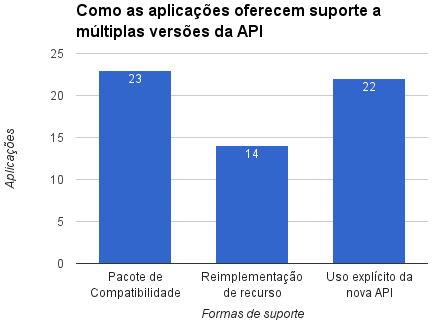
\includegraphics[scale=0.75]{imagens/forma_suporte}
  	\textsf{\caption{Como as aplicações oferecem suporte a múltiplas versões da API}
  	        \label{fig:forma_suporte}}
\end{figure}

A técnica de uso explícito da nova API pode causar um erro na aplicação caso seja
executado em um dispositivo com versão da API inferior àquela em que o componente
utilizado foi adicionado. Assim, é necessário algum mecanismo para evitar que isso
aconteça. O mecanismo primário padrão é um comando condicional. No entanto, existem
diversas maneiras de implementação de tal comando condicional, desde uma instrução
\texttt{if} logo acima da linha de código, até a utilização de padrões de projeto,
em que o \texttt{if} determina a criação de objetos baseado na versão da API Android
do dispositivo, por exemplo.

O gráfico apresentado na figura \ref{fig:alternativas_EC} mostra as diferentes
alternativas de projeto encontradas nas aplicações analisadas para implementação
de execução condicional em torno das linhas com ocorrências de Lint NewApi. Tais
resultados foram obtidos a partir da análise do resultado da execução do Lint NewApi
nas aplicações. Execução condicional \cite{Santos2012} indireta e uso de padrões
de projeto foram as técnicas mais comum, estando presente em 16 aplicações analisadas.
Execução condicional direta e suporte implícito foram utilizadas em 12 aplicações cada.
6 aplicações deixaram de fazer o tratamento de algumas ocorrências, 5 aplicações possuem ocorrências dentro de métodos que nunca serão executados e, por fim, uma aplicação
utilizou tratamento de exceção para evitar erro durante a execução.

\begin{figure}[htb]
	\centering 
  	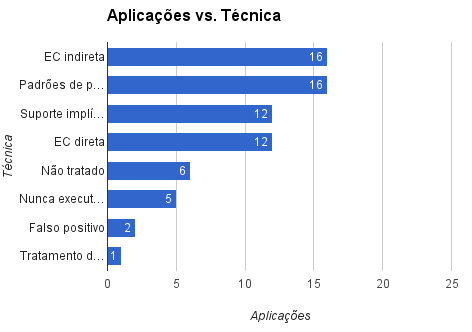
\includegraphics[scale=0.75]{imagens/alternativas_EC}
  	\textsf{\caption{ Quantidade de aplicações que utilizaram cada técnica para
  						tratamento de ocorrência de NewApi}
  	        \label{fig:alternativas_EC}}
\end{figure}

Também foram detectadas ocorrências de falsos positivos em duas aplicações.
Falso positivo acontece quando um determinado método \texttt{X()} qualquer foi
adicionado em uma classe da API em versão superior da aplicação, posteriormente
uma classe estende essa classe da API e implementa o método \texttt{X()}, mas
o Lint NewApi não identifica essa implementação, reportando o falso problema.

A figura \ref{fig:falso_positivo} exemplifica tal situação com um dos casos reais 
encontrados. O método \texttt{invalidadeOptionsMenu()} foi adicionado à classe
\texttt{Activity} na versão 11 da API, portanto ele não pode ser chamado em
versões anteriores. Assim, foi disponibilizado através da re-implementação na classe 
\texttt{AppCompatActivity} do pacote de compatibilidade e que herda de \texttt{Activity}.
Na aplicação Telegram, cuja API mínima é 10, existe uma classe que estende de 
\texttt{AppCompatActivity}, \texttt{CastEnableActivity}, que é então estendida por 
\texttt{MediaPlayerActivity}. No método \texttt{onOptionsItemSelected()} é feita 
uma chamada para \texttt{invalidadeOptionsMenu()}. Tal chamada é indevidamente
indicada pelo Lint.

\begin{figure}[htb]
	\centering 
  	\includegraphics[scale=0.6]{imagens/falso_positivo}
  	\textsf{\caption{Diagrama de classe exemplificando situação de falso positivo do Lint}
  	        \label{fig:falso_positivo}}
\end{figure}

A figura \ref{fig:percentuais_forma_tratamento} apresenta os percentuais das
formas de tratamento para as ocorrências de NewAPI. Foram analisadas um total
de 1556 ocorrências de NewAPI. Desse total, 40,6\% foi tratado com EC indireta,
22,8\% com algum padrão de projeto, 18,9\% através de EC direta, 10,7\% utilizando
suporte implícito da plataforma, 5,3\% das ocorrências não foram devidamente tratadas.
Esses dois últimos casos são situações críticas, merecedoras de uma maior atenção.
A primeira por depender de um conhecimento mais específico da API, para identificar
que a chamada não será executada em versões antigas. A última por ser fonte de bugs
nas aplicações. Continuando a análise, 1,2\% das ocorrências estão dentro de métodos
que nunca serão executados e, por fim, duas pequenas frações de 0,3\% das ocorrências
foi utilizada tratamento de exceção ou são falsos positivos. Essas ocorrências de NewAPI 
estão distribuídas em 22 aplicações (3 aplicações não apresentaram ocorrências de alguma 
NewAPI).

\begin{figure}[htb]
	\centering 
  	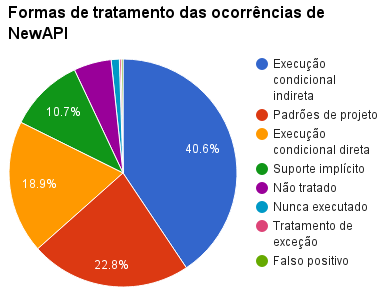
\includegraphics[scale=0.75]{imagens/percentuais_forma_tratamento}
  	\textsf{\caption{Percentuais de formas de tratamento das ocorrências de NewAPI}
  	        \label{fig:percentuais_forma_tratamento}}
\end{figure}

O figura \ref{fig:padroes_por_aplicacao} apresenta os padrões de projeto utilizados
por quantidade de aplicações. O padrão \textit{Strategy} é o que mais foi utilizado
em um total de 12 aplicações. \textit{Template Method} e \textit{Null Object} foram 
utilizados por uma aplicação cada um. \textit{Proxy} foi utilizado por duas aplicações. Apenas uma aplicação utilizou dois padrões de projetos simultaneamente, \textit{Strategy}
e \textit{Proxy}. 

\begin{figure}[htb]
	\centering 
  	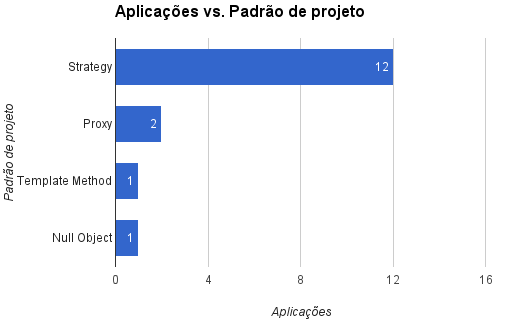
\includegraphics[scale=0.75]{imagens/padroes_por_aplicacao}
  	\textsf{\caption{Quantidade de aplicações que utilizaram padrões de projeto para
  						tratar ocorrências de NewApi}
  	        \label{fig:padroes_por_aplicacao}}
\end{figure}

O figura \ref{fig:percentuais_por_padrao} apresenta os percentuais dos padrões de
projeto utilizados como forma de tratamento para as ocorrências de NewAPI. Do total
de 1554 ocorrências de NewAPI analisadas, 355 (22,8\%) foram tratadas com algum
padrão de projeto. Sendo o mais comum o padrão \textit{Strategy}, responsável por
77,7\% (276) desse total. Os padrões \textit{Proxy} e \textit{Template Method}
foram responsáveis por 19,4\% e 2,3\% dos casos, respectivamente. \textit{Null Object}
foi utilizado por uma aplicação para tratar 2 (0,6\%) ocorrências.

\begin{figure}[htb]
	\centering 
  	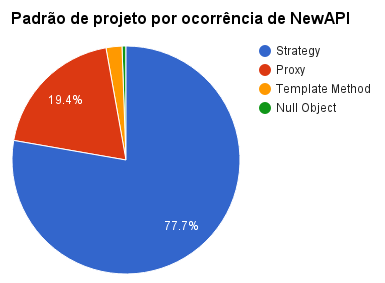
\includegraphics[scale=0.75]{imagens/percentuais_por_padrao}
  	\textsf{\caption{Percentuais de uso de padrões de projeto por ocorrências de NewAPI}
  	        \label{fig:percentuais_por_padrao}}
\end{figure}

\subsection{Qual o subconjunto de novas funcionalidades da plataforma que são
mais utilizados por aplicações compatíveis com versões antigas da API?}

Analisamos as chamadas às novas APIs para determinar o subconjunto das
novas funcionalidades que são utilizadas pelas aplicações com suporte à versões
antigas da API. Os resultados foram contabilizados em função da taxonomia da API.
E, então, para as taxonomias mais comuns, apresentamos as classes mais recorrentes. 

\subsubsection{Pacote de Compatibilidade}

Para computar os dados relativos à pacote de compatibilidade, realizamos uma análise
estática sobre os projetos, identificando nos trechos de importação das classes Java
os elementos advindos do pacote \texttt{android.support}, excetuando os subpacotes
\texttt{annotations} e \texttt{tests}, pois estes além de não influenciarem na execução
da aplicação, não são analisadas pelo Lint NewApi. Os resultados foram contabilizados
em função da taxonomia da API. E então, para as taxonomias mais comuns, apresentamos
as classes mais recorrentes.

A tabela \ref{tab:elementos_pacote} apresenta os valores obtidos. Para cada taxonomia,
temos o número de aplicações que fizeram \texttt{import}’s do pacote de compatibilidade,
o total de \texttt{import}’s feitos, as importações únicas e a média de \texttt{import}’s 
por aplicação. Importações únicas significa que se uma classe é importada mais de uma vez, 
independente de aplicação, ela é contabilizado apenas uma vez. Em destaque os maiores 
valores de cada coluna, além das duas taxonomias mais significativas, que possuem uma
 maior média de \texttt{import}’s por aplicação.

\begin{table}[!htbp] % TODO posicionar melhor essa tabela
  \centering
  \caption{Elementos mais utilizados do pacote de compatibilidade}
  \begin{tabular}{| l | r | r | r | r |}
  	\hline
  	% rótulo das columnas
  	\multicolumn{1}{|c|}{\textbf{Taxonomia}} &
  	\multicolumn{1}{c|}{\textbf{Aplicações (A)}} &
 	\begin{tabular}[c]{@{}c@{}}
 		\textbf{Total de}\\ \textbf{import's (B)}
 	\end{tabular} &
 	\begin{tabular}[c]{@{}c@{}}\textbf{Importações}\\ \textbf{unicas}\end{tabular} &
 	\begin{tabular}[c]{@{}c@{}}\textbf{Média por}\\ \textbf{app (A/B)}\end{tabular} \\ \hline
 	%dados
 	animation 		& 1 			& 5   			&   4 			& 5  \\ \hline
 	\textbf{app}	& \textbf{22} 	& \textbf{849}  &  49 			& \textbf{39}\\ \hline
 	content 		& 17 			& 236 			&  11 			& 14  \\ \hline
 	graphics  		& 4 			& 9 			&   5 			& 2  \\ \hline
 	hardware   		& 1 			& 2 			&   1 			& 2  \\ \hline
 	media    		& 3 			& 15 			&   7 			& 5  \\ \hline
 	net     		& 1 			& 3   			&   1 			& 3  \\ \hline
 	os      		& 3 			& 6   			&   4 			& 2  \\ \hline
 	preference  	& 5 			& 99   			&  17 			& 20  \\ \hline
 	provider    	& 1 			& 12 			&   1			& 12   \\ \hline
 	text        	& 1 			& 1 			&   1 			& 1   \\ \hline
 	util       	 	& 9 			& 46 			&   9 			& 5   \\ \hline
 	view        	& 18 			& 233 			&  37 			& 13   \\ \hline
 	\textbf{widget} & 18			& 410 			&  \textbf{65} 	& 23   \\ \hline
  \end{tabular}
  \label{tab:elementos_pacote}
\end{table}

As taxonomias \textit{app} e \textit{widget} são as mais comuns. A primeira contém
classes de alto nível que encapsulam o modelo geral de aplicações Android. A última
fornece elementos de interface com o usuário para serem utilizados na tela da aplicação.

\textit{App} possui o maior número importações, 849, e também maior média por aplicação,
39, distribuídos em 22 das 25 aplicações analisadas. Já \textit{widget} possui um número
bem menor
de importações, 410, embora bem mais alto que a terceira posição. Estando distribuídos em
18 aplicações. Além de possuir o maior número de chamadas únicas, 65. Isso demonstra que
os elementos de \textit{app} são mais restritos, enquanto \textit{widget} há uma
granularidade maior, havendo um maior acoplamento da aplicação a esses elementos em
relação aos elementos de \textit{app}.

Da taxonomia \textit{app}, a classe mais comum é \texttt{Fragment}, conforme apresenta
a tabela \ref{tab:elementos_app}. Além disso, outras três classes diretamente relacionadas
a fragmentos estão entre as 10 mais utilizadas: \texttt{DialogFragment}, 
\texttt{FragmentManager} e \texttt{FragmentActivity}.

\begin{table}[!htbp] % TODO posicionar melhor essa tabela
  \centering
  \caption{10 classes da taxonomia \textit{app} mais importadas do pacote de compatibilidade}
  \begin{tabular}{| l | r | r | r | }
  	\hline
  	% rótulo das columnas
  	\multicolumn{1}{|c|}{\textbf{Classes}} &
  	\multicolumn{1}{c|}{\textbf{Aplicações (A)}} &
 	\begin{tabular}[c]{@{}c@{}}
 		\textbf{Total de}\\ \textbf{importações (B)}
 	\end{tabular} &
 	\begin{tabular}[c]{@{}c@{}}\textbf{Média por}\\ \textbf{app (B/A)}\end{tabular} \\ \hline
 	%dados
 	v4.app.Fragment 			& 15 			& 144   		&   10 			  \\ \hline
 	v4.app.NotificationCompat	& 16 			& 80 			&   5 			  \\ \hline
 	v4.app.DialogFragment  		& 12 			& 76   			&   6 			  \\ \hline
 	v7.app.AlertDialog     		& 11 			& 72   			&   7			  \\ \hline
 	v7.app.AppCompatActivity  	& 14 			& 67   			&  5 			  \\ \hline
 	v4.app.FragmentManager    	& 16 			& 65 			&   4			   \\ \hline
 	v4.app.FragmentActivity    	& 12 			& 58 			&   5 			   \\ \hline
 	v4.app.LoaderManager       	& 7 			& 50 			&   5 			   \\ \hline
 	v7.app.ActionBar        	& 13 			& 37 			&  3 			   \\ \hline
 	v4.app.ActivityCompat 		& 14			& 25 			&  2 	   \\ \hline
  \end{tabular}
  \label{tab:elementos_app}
\end{table}

Se na taxonomia \textit{app} as importações tendem a elementos relacionados a
fragmentos, na taxonomia \textit{widget} houve uma maior dispersão. As classes
mais comuns são \texttt{RecyclerView} e \textit{Toolbar}. A primeira teve o
maior número de importações no total, enquanto a segunda, além de ter o segundo
maior valor de importações, é a que está presente em mais aplicações, 12 contra
9 para \textit{RecyclerView}. Os demais elementos aparecem em no máximo 9 aplicações,
com não mais que 26 importações no total. A tabela \ref{tab:elementos_widget}
apresenta as 10 classes da taxonomia \textit{widget} mais utilizadas.

\begin{table}[!htbp] % TODO posicionar melhor essa tabela
  \centering
  \caption{10 classes da taxonomia \textit{widget} mais importadas do pacote de compatibilidade}
  \begin{tabular}{| l | r | r | r | }
  	\hline
  	% rótulo das columnas
  	\multicolumn{1}{|c|}{\textbf{Classes}} &
  	\begin{tabular}[c]{@{}c@{}}
  	 		\textbf{Aplicações}\\ \textbf{(A)}
  	 	\end{tabular} &
 	\begin{tabular}[c]{@{}c@{}}
 		\textbf{Total de}\\ \textbf{importações (B)}
 	\end{tabular} &
 	\begin{tabular}[c]{@{}c@{}}\textbf{Média por}\\ \textbf{app (B/A)}\end{tabular} \\ \hline
 	%dados
 	v7.widget.RecyclerView 				& 9 	& 81 	  		&   9 			  \\ \hline
 	v7.widget.Toolbar					& 12 	& 52 			&   4 			  \\ \hline
 	v7.widget.LinearLayoutManager		& 9 	& 26   			&   3 			  \\ \hline
 	design.widget.Snackbar     			& 6 	& 23   			&   4			  \\ \hline
 	v7.widget.SearchView  				& 8		& 21   			&   3 			  \\ \hline
 	v4.widget.DrawerLayout    			& 9 	& 15 			&   2			   \\ \hline
 	design.widget.FloatingActionButton  & 4		& 13 			&   3 			   \\ \hline
 	v7.widget.PopupMenu       			& 5 	& 12 			&   2 			   \\ \hline
 	design.widget.TabLayout        		& 6		& 10 			&   3 			   \\ \hline
 	v4.widget.SwipeRefreshLayout 		& 5		& 10 			&   2 	   \\ \hline
  \end{tabular}
  \label{tab:elementos_widget}
\end{table}


\subsubsection{Re-implementação de Recursos}

Re-implementação de um recurso existente na API padrão pode ser uma re-implementação
completamente própria, quando não existe cópia de código de outros projetos, ou pode
ser através da cópia do código-fonte do recurso na API padrão. Para este trabalho,
consideramos apenas a re-implementação através de cópia do código-fonte da API padrão.
O código-fonte do projeto Android é distribuído, preferencialmente, sob a licença Apache 
Software License, Versão 2.0 ("Apache 2.0") \cite{License}, e os direitos autorais
pertencem a \textit{Android Open Source Project}. Para indicar isso, todos os arquivos
do projeto possuem o seguinte preâmbulo:
\texttt{
\newline
/* \newline
 * Copyright (C) <YEAR> The Android Open Source Project \newline
 * \newline
 * Licensed under the Apache License, Version 2.0 (the "License"); \newline
 * you may not use this file except in compliance with the License. \newline
 * You may obtain a copy of the License at \newline
 * \\
 *      http://www.apache.org/licenses/LICENSE-2.0 \\
 * \\
 * Unless required by applicable law or agreed to in writing, software \\
 * distributed under the License is distributed on an "AS IS" BASIS, \\
 * WITHOUT WARRANTIES OR CONDITIONS OF ANY KIND, either express or implied. \\
 * See the License for the specific language governing permissions and \\
 * limitations under the License. \\
 */
} 

Assim, para verificarmos se o as aplicações re-implementaram algum recurso através
da cópia de código da API padrão, realizamos uma busca textual nos arquivos Java
das aplicações por "Android Open Source Project". Para cada ocorrência, era feita
uma pesquisa na documentação da API pelo nome da classe. Se não fosse encontrado
algo, era feita uma busca no Google, pela string "android <nome da classe>".
Analisamos as ocorrências  para determinar se o código havia sido copiado realmente
da API, de aplicações nativas do Android ou de projeto de exemplos oficiais,
desenvolvidas pela mesma equipe da plataforma. Em algumas situações, os códigos
tinham como origem o projeto Android, mas não faziam parte da API. Um exemplo disso
é a classe \texttt{NetworkActivity} que, embora desenvolvida pelo projeto Android e
possuir o preâmbulo citado acima, não faz parte da API. Ela é apresentada na
documentação \cite{NetworkUsage} e o código-fonte está no subdiretório \texttt{samples}
do repositório \cite{NetworkActivity}. Ocorrências como essa eram então descartadas.
Embora um número considerável de aplicações (14 de 25) tenha utilizado tal técnica,
foram usos bem pontuais e localizadas.

O conjunto de classes mais significativo diz respeito à implementação do pacote 
\texttt{android.animation} da API e ocorreu em 3 aplicações. O código presente
nas aplicações é proveniente da biblioteca NineOldAndroids\footnote{http://nineoldandroids.com/},
que disponibiliza seus arquivos para
download através do código-fonte e não em arquivos JAR ou algum outro mecanismo
para adição de dependência aos projetos, mas que isole o código da dependência
do código principal do projeto. Por esse motivo, tal código foi considerado
nessa análise. As classe \texttt{PreferenceFragment} e \texttt{PreferenceManager}
foram também re-implementadas por 3 aplicações.

A classe \texttt{android.util.Base64}, utilizada para codificação e decodificação
da representação de dados binários em Base64 \cite{RFC4648}, foi a classe mais
recorrente, detectada em 5 aplicações. Outras mais de 30 classes com propósitos 
diversos também foram re-implementadas, no entanto, em não mais de uma aplicação.

Tal cenário, aponta que re-implementação de recursos é utilizada quando se deseja
poucos e pontuais recursos adicionais. Sendo mais vantajoso copiar o código-fonte
da API, do que usar pacote de compatibilidade, caso o recurso também seja
disponibilizado dessa forma. Além disso, só é possível tal mecanismo, pelo menos em
relação ao código da API oficial, devido ao fato de ser \textit{open-source} e a
licença permitir cópia, alteração e redistribuição do código-fonte.

\subsubsection{Uso explícito da nova API}

Para determinar o subconjunto das novas funcionalidades da API que são utilizadas
pelas aplicações com suporte a versões antigas da API através de uso explícito da
nova API, processamos os resultados da saída do Lint NewApi. Os resultados foram contabilizados em função da taxonomia da API. E então, para as taxonomias mais
comuns, apresentamos as classes mais recorrentes.

A tabela \ref{tab:elementos_nova_api} apresenta os valores obtidos. Para cada
taxonomia, temos a quantidade total de ocorrências de NewApi, o número de
ocorrências únicas, a quantidade de aplicações em que as ocorrências apareceram
e a média de ocorrências por aplicação.

\begin{table}[!htbp] % TODO posicionar melhor essa tabela
  \centering
  \caption{Ocorrências de NewApi por taxonomia}
  \begin{tabular}{| l | r | r | r | r |}
  	\hline
  	% rótulo das colunas
  	\multicolumn{1}{|c|}{\textbf{Taxonomia}} &
  	\begin{tabular}[c]{@{}c@{}}
  	 		\textbf{Ocorrências de}\\ \textbf{NewApi (A)}
  	\end{tabular} &
  	\begin{tabular}[c]{@{}c@{}}
 		\textbf{Ocorrências}\\ \textbf{Únicas}
 	\end{tabular} &
 	\textbf{Aplicações (B)} &
 	\begin{tabular}[c]{@{}c@{}}
 		\textbf{Média por}\\ \textbf{app (A/B)}
 	\end{tabular} \\ \hline
 	%dados
 	animation 		& 149 			& 29   			&   7 			& 21.29  \\ \hline
 	\textbf{app}	& \textbf{360} 	& 57   			&  16 			& 22.50 \\ \hline
 	appwidget 		& 5 			& 0!!!   		&   2 			& 2.50  \\ \hline
 	content 		& 44 			& 24 			&  11 			& 4.00  \\ \hline
 	database 		& 10 			& 8   			&  4  			& 2.50  \\ \hline
 	graphics  		& 26 			& 14 			&   6 			& 4.33  \\ \hline
 	hardware   		& 3 			& 3 			&   1 			& 3.00  \\ \hline
 	media    		& 190 			& 54 			&   3 			& \textbf{63.33}  \\ \hline
 	net     		& 31			& 12   			&   2 			& 15.50  \\ \hline
 	nfc      		& 14 			& 7   			&   2 			& 7.00  \\ \hline
 	opengl      	& 25 			& 17   			&   1 			& 25.00  \\ \hline
 	os      		& 82 			& 20   			&   9 			& 9.11  \\ \hline
 	preference  	& 56			& 4   			&   5 			& 11.20  \\ \hline
 	print    		& 10 			& 7 			&   1			& 10.00   \\ \hline
 	provider    	& 27			& 15 			&   7			& 3.86   \\ \hline
 	service        	& 4 			& 2 			&   1 			& 4.00   \\ \hline
 	speech        	& 3 			& 2 			&   1 			& 3.00   \\ \hline
 	telephony       & 29 			& 25 			&   2 			& 14.50   \\ \hline
 	text        	& 6 			& 5 			&   5 			& 1.20   \\ \hline
 	transition 	 	& 4 			& 1 			&   1 			& 4.00   \\ \hline
 	util       	 	& 8				& 3 			&   2 			& 4.00   \\ \hline
 	view        	& 353 			& \textbf{153} 	&  \textbf{20} 	& 17.65   \\ \hline
 	webkit        	& 11 			& 7 			&  4 			& 2.75   \\ \hline
 	widget 			& 92			& 41 			&  10 			& 9.20   \\ \hline
 	java.io 		& 3				& 2 			&  2 			& 1.50   \\ \hline
 	java.lang 		& 3				& 2 			&  2 			& 1.50   \\ \hline
 	java.net 		& 5				& 4 			&  1 			& 5.00   \\ \hline
 	java.util 		& 1				& 1 			&  1 			& 1.00   \\ \hline
  \end{tabular}
  \label{tab:elementos_nova_api}
\end{table}

As taxonomias \textit{app} e \textit{view} foram as mais comuns nas aplicações analisadas.
A primeira contém classes de alto nível que encapsulam o modelo geral de aplicações Android.
A última fornece classes básicas para interface com usuário, relacionadas a layout das telas
e interação com usuário. \textit{App} e \textit{view} possuem os maiores número de ocorrências
de NewApi, 360 e 353, respectivamente. Ocorrências em arquivos XML foram contabilizados também,
tendo um total de 50 ocorrências. No entanto, a maior média por aplicação pertence a taxonomia
\textit{media}, no valor de 63,33, distribuídos em 3 aplicações:  VLC, Firefox e Telegram.
Enquanto \textit{app} e \textit{view} estão distribuídas em 16 e 20 aplicações, respectivamente.

Tais valores refletem o objetivo das taxonomias e a categoria das aplicações.
\textit{App} e \textit{view} contém classes utilizadas em qualquer aplicação, enquanto que a
taxonomia \textit{media} mantém classes relacionadas a multimídia. Mais úteis para um reprodutor
e editor de vídeos (VLC), um navegador web (Firefox) e um aplicativo de comunicação (Telegram)
com recursos de reprodução de multimídia (imagem, som e vídeo) embutido.

A tabela \ref{tab:newapi_app} apresenta os elementos da taxonomia app com maior
números de ocorrência de NewApi agrupados pelo elemento de maior granularidade
que surgiu na versão da API indicada por NewApi. Assim, todas as classes do pacote
\texttt{android.app.backup} foram agrupadas pelo pacote porque o próprio pacote
surgiu apenas na versão 5. A classe \texttt{android.app.Fragment} surgiu na versão
11, então agrupamos aqui todos os seus métodos. Já a classe \texttt{android.app.Activity}
existe desde a versão 1 e foram diversos métodos novos apontados por NewApi. Na
classe \texttt{android.app.Notification}, que existe desde a versão 1, apenas o
método \texttt{bigContentView} é apontado por NewApi.

\begin{table}[!htbp] % TODO posicionar melhor essa tabela
  \centering
  \caption{Elementos da taxonomia app com ocorrências de NewApi}
  \begin{tabular}{| l | r | r |}
  	\hline
  	% rótulo das colunas
  	\multicolumn{1}{|c|}{\textbf{Descrição}} &
  	\begin{tabular}[c]{@{}c@{}}
  	 		\textbf{Ocorrências de}\\ \textbf{NewApi (A)}
  	\end{tabular} &
  	\textbf{Aplicações} \\ \hline
 	%dados
 	\textbf{Classe android.app.Fragment}			& 188 	& 2 \\ \hline
 	Pacote android.app.backup						& 36	& 4 \\ \hline
 	Métodos de android.app.Activity 				& 30 	& 8 \\ \hline
 	Classe android.app.Presentation 				& 28 	& 2  \\ \hline
 	Método android.app.Notification\#bigContentView	& 17 	& 1  \\ \hline
 	Classe android.app.ActionBar  					& 12 	& 3 \\ \hline
 	Classe android.app.Notification.Builder   		& 10 	& 1 \\ \hline
 	\textbf{Classe android.app.FragmentTransaction}	& 9 	& 2  \\ \hline
 	Classe android.app.DownloadManager     			& 9		& 1   \\ \hline
 	\textbf{Classe android.app.FragmentManager}    	& 7		& 2   \\ \hline
  \end{tabular}
  \label{tab:newapi_app}
\end{table}

Da taxonomia \textit{app}, a classe mais comum é \texttt{Fragment}, conforme
apresentado na tabela \ref{tab:newapi_app}. Além disso, alguns métodos da classe
\texttt{Activity} nessa relação são relacionadas aos fragmentos, assim como as
classes \texttt{FragmentTransaction} e \texttt{FragmentManager}. Além dos elementos
apresentados na tabela \ref{tab:newapi_app}, outros 7 elementos possuem um valor
máximo de 4 ocorrências relacionadas.

Se as ocorrências para a taxonomia \textit{app} ficaram concentradas em elementos
relacionados a fragmentos, na taxonomia \textit{view} houve uma maior dispersão.
A classe mais comum, tanto em aplicações (12) quanto em ocorrências de NewApi (108),
é a classe \texttt{View}, classe base para todos os componentes de construção de
interface gráfica. Atributos ou tags XML correspondem a 50 ocorrências, distribuídas
em 7 aplicações. Os demais elementos, aparecem em no máximo 4 aplicações, o que
demonstra serem específico do tipo de aplicação. Por exemplo, as classes
\texttt{InputMethodSubtype} e \texttt{InputMethodManager} juntas somam 12 ocorrências
de NewApi, mas todas elas em uma única aplicação, a AnySoftKeyboard, uma aplicação de
teclado virtual. 

A tabela \ref{tab:newapi_view} apresenta os 10 elementos da taxonomia \textit{view}
com mais ocorrência de NewApi. Além desses, outros 20 elementos apresentam no máximo
6 ocorrências.

\begin{table}[!htbp] % TODO posicionar melhor essa tabela
  \centering
  \caption{10 elementos da taxonomia view com mais ocorrência de NewApi}
  \begin{tabular}{| l | r | r |}
  	\hline
  	% rótulo das colunas
  	\multicolumn{1}{|c|}{\textbf{Descrição}} &
  	\begin{tabular}[c]{@{}c@{}}
  	 		\textbf{Ocorrências de}\\ \textbf{NewApi}
  	\end{tabular} &
 	\textbf{Aplicações} \\ \hline
 	%dados
 	Métodos de android.view.View							& 108 	& 12 \\ \hline
 	Atributos ou tags XML									& 50	& 7 \\ \hline
 	Classe android.view.ViewPropertyAnimator 				& 43 	& 2 \\ \hline
 	Classe android.view.WindowInsets 						& 23 	& 1  \\ \hline
 	Classe android.view.TextureView							& 21 	& 2  \\ \hline
 	Classe android.view.ScaleGestureDetector  				& 12 	& 3 \\ \hline
 	Classe android.view.ActionMode   						& 11 	& 3 \\ \hline
 	Métodos de android.view.MotionEvent						& 10 	& 1  \\ \hline
 	Construtor de android.view.ViewOutlineProvider     		& 10	& 1   \\ \hline
 	Classe android.view.accessibility.AccessibilityNodeInfo & 9		& 1   \\ \hline
  \end{tabular}
  \label{tab:newapi_view}
\end{table}

Tanto os elementos relacionados a fragmentos, quanto a grande maioria dos métodos
da classe \texttt{View} citados anteriormente surgiram na versão 11 da API, e foram
uma importante melhoria na plataforma, o que reforça o alto índice de ocorrências de
NewApi relacionado a esta versão, conforme apresentado no figura \ref{fig:newapi_por_versao}.
Tais ocorrências estão distribuídas em 18 aplicações. 

\begin{figure}[htb]
	\centering 
  	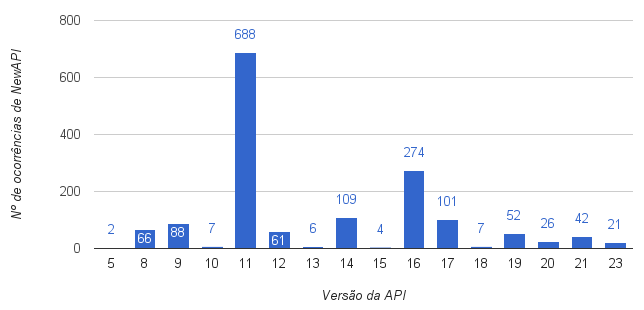
\includegraphics[scale=0.6]{imagens/newapi_por_versao}
  	\textsf{\caption{Nº de ocorrências de NewApi por versão da API}
  	        \label{fig:newapi_por_versao}}
\end{figure}

\subsection{Qual o esforço necessário para aumentar a compatibilidade com um
maior número de API's de versões anteriores da plataforma?}

Definir um valor de API mínima para execução da aplicação, significa deixar de
atender todos os aparelhos com API inferior. Em algumas situações, isso pode
representar uma perda do mercado potencial. Assim, analisamos qual seria o esforço
para aumentar a compatibilidade com um maior número de API's. Para tal, editamos o
código-fonte da aplicação (arquivos \texttt{build.gradle} ou \texttt{AndroidManifest.xml},
conforme o caso) e re-executamos o Lint NewApi. Então comparamos o resultado aqui
obtido com o resultado obtido na versão original.

Inicialmente, identificamos a quantidade de novas ocorrências de NewApi que
surgiam com a diminuição da versão da API. Isso fornece um valor quantitativo
do trabalho necessário para aumento da compatibilidade, quanto maior este valor
mais adequações seriam necessárias no código-fonte. A tabela \ref{tab:esforco}
apresenta tais resultados. Para cada aplicação, indicamos situação atual, com
a API mínima atual e a quantidade de ocorrências de NewApi, a situação após nova
edição, com a nova API e a quantidade de ocorrências de NewApi, e a diferença de 
ocorrência de NewApi, com a diferença total de novas ocorrências e dessas a quantidade
de ocorrências únicas. Essas duas últimas colunas mensuram quantitativamente o esforço
necessário para aumentar a compatibilidade.   

% Please add the following required packages to your document preamble:
% \usepackage{multirow}
\begin{table}[!htbp]
\fontsize{9}{11}
\centering
\caption{Esforço quantitativo para aumentar compatibilidade com mais versões da API}
\label{tab:esforco}
\begin{tabular}{|l|r|r|r|r|r|r|}
\hline
\multicolumn{1}{|c|}{\multirow{2}{*}{\textbf{Aplicação}}}                & \multicolumn{2}{c|}{\textbf{Situação atual}}                                                                                                                                       & \multicolumn{2}{c|}{\textbf{Situação após edição}}                                                                                                                                 & \multicolumn{2}{c|}{\textbf{\begin{tabular}[c]{@{}c@{}}Diferenças de\\ ocorrências\\ de NewAPI\end{tabular}}}                                                                          \\ \cline{2-7} 
\multicolumn{1}{|c|}{}                                                   & \multicolumn{1}{c|}{\textbf{\begin{tabular}[c]{@{}c@{}}API\\ Mínima\end{tabular}}} & \multicolumn{1}{l|}{\textbf{\begin{tabular}[c]{@{}l@{}}Ocorrências\\ de NewApi\end{tabular}}} & \multicolumn{1}{c|}{\textbf{\begin{tabular}[c]{@{}c@{}}API\\ Mínima\end{tabular}}} & \multicolumn{1}{l|}{\textbf{\begin{tabular}[c]{@{}l@{}}Ocorrências\\ de NewApi\end{tabular}}} & \multicolumn{1}{c|}{\textbf{\begin{tabular}[c]{@{}c@{}}Diferen\\ ça total\end{tabular}}} & \multicolumn{1}{c|}{\textbf{\begin{tabular}[c]{@{}c@{}}Ocorrên\\ cias únicas\end{tabular}}} \\ \hline
\begin{tabular}[c]{@{}l@{}}Numix Circle\\ icon pack\end{tabular}         & 16                                                                                 & 0                                                                                             & 15                                                                                 & 1                                                                                             & 1                                                                                        & 1                                                                                           \\ \hline
SnoopSnitch                                                              & 16                                                                                 & 19                                                                                            & 15                                                                                 & 15                                                                                            & 2                                                                                        & 1                                                                                           \\ \hline
\begin{tabular}[c]{@{}l@{}}Yaaic -\\ IRC Client\end{tabular}             & 21                                                                                 & 0                                                                                             & 15                                                                                 & 1                                                                                             & 1                                                                                        & 1                                                                                           \\ \hline
\begin{tabular}[c]{@{}l@{}}Hangar -\\ Smart app\\ shortcuts\end{tabular} & 16                                                                                 & 14                                                                                            & 15                                                                                 & 21                                                                                            & 7                                                                                        & 5                                                                                           \\ \hline
\begin{tabular}[c]{@{}l@{}}WiFi\\ Analyzer\end{tabular}                  & 22                                                                                 & 0                                                                                             & 21                                                                                 & 1                                                                                             & 1                                                                                        & 1                                                                                           \\ \hline
AcDisplay                                                                & 16                                                                                 & 167                                                                                           & 15                                                                                 & 193                                                                                           & 26                                                                                       & 10                                                                                          \\ \hline
\begin{tabular}[c]{@{}l@{}}Indic\\ Keyboard\end{tabular}                 & 16                                                                                 & 7                                                                                             & 15                                                                                 & 14                                                                                            & 11                                                                                       & 5                                                                                           \\ \hline
\begin{tabular}[c]{@{}l@{}}DashClock\\ Widget\end{tabular}               & 17                                                                                 & 5                                                                                             & 16                                                                                 & 46                                                                                            & 41                                                                                       & 9                                                                                           \\ \hline
Termux                                                                   & 21                                                                                 & 2                                                                                             & 19                                                                                 & 59                                                                                            & 57                                                                                       & 9                                                                                           \\ \hline
\end{tabular}
\end{table}

Posteriormente, analisamos cada uma dessas ocorrências para identificar como ela
poderia ser tratada e qual o impacto para a aplicação. Das 10 aplicações analisadas,
5 delas podem aumentar a compatibilidade com poucos e simples ajustes, fazendo uso
de pacote de compatibilidade e/ou execução condicional, sem perda de funcionalidade.
Quatro dessas aplicações, poderiam passar a exigir API 15, no lugar da atual 16. Mas
uma delas, Yaaic, poderia substituir a API 21 pela API 15, com apenas 1 ocorrência de
NewApi a mais. Tal ocorrência existe devido ao uso do tema Material\cite{Material}, que pode ser tratado através do mecanismos de recursos da plataforma, bastando definir estilos gerais, para versões inferiores a 21, e um estilo específico (style-v21) para versão 21 ou superior. Nesta aplicação, também é possível ir além, e prover compatibilidade com a versão 10 da API. Em que 8 novas ocorrências de NewApi surgiriam, mas poderiam ser resolvidas com pacote de compatibilidade.

Outras 2 aplicações - Indic Keyboard e AcDisplay - precisam tratar, respectivamente,
9 e 26 novas ocorrências de NewApi para alterar a API de 16 para 15. A primeira teria
que apenas fazer uma re-implementação da classe \texttt{SentenceSuggestionsInfo},
surgida na API 16. Todas as 9 ocorrências de NewApi são referências para essa classe.
A segunda teria que tomar providências diversas, como pacote de compatibilidade, execução
condicional e re-implementação de recursos. Mas todas elas possíveis de resolução sem perda
de funcionalidade na aplicação.

As três aplicações restantes usam funcionalidades mais críticas. Focal, uma
aplicação de fotografia, apresenta um total de 11 ocorrências, sendo que uma
delas parece não haver solução possível, pois depende de suporte do hardware
do aparelho para auto focus da câmera. DashClock Widget apresentou 41 novas
ocorrências ao reduzir a versão da API de 17 para 16. A maioria pode ser
resolvida pelos métodos já citados, 17 delas são referências a classe
\texttt{DreamService}, uma classe específica para realidade virtual.
Portanto, a aplicação poderia fornecer as demais funções mas omitir esta
específica. Por fim, a aplicação Termux, um emulador de terminal, é a que
possui a maior quantidade de ocorrências de NewApi, ao reduzir a versão da
API de 21 para 19: 57 ocorrências. A maioria facilmente tratada pelos métodos
já citados. Porém, 9 delas fizerem referência a classe \texttt{android.system.Os},
as quais são funcionalidades fundamentais para a aplicação, de acesso ao sistema.
Distribuir a aplicação sem tais recursos seria uma perda considerável. Essa classe
expõe para a API pública do Android uma classe pertencente ao pacote \texttt{libcore},
o qual não pode ser importado pelas classes das aplicações da mesmo forma que classes
do pacote \texttt{android}. No entanto, é possível através de uma re-implementação de
recurso mais elaborada que as citadas anteriormente, usando reflexão, acessar tal pacote
e classes internas \cite{Libcore}, e então fazer uma implementação própria da classe Os,
ainda que fazer uso de APIs internas seja uma má prática de programação e existam
recomendações contrárias à sua adoção \cite{Businge2015} \cite{Mastrangelo2015}.

A tabela \ref{tab:esforco_resumo} resume o resultado qualitativo, agrupando as aplicações
em três níveis de dificuldade e possíveis soluções para as novas ocorrências de NewApi.
Os resultados encontrados, associado à tabela de distribuição das versões (figura 
\ref{fig:platform_versions}), apresenta evidências de que as aplicações poderiam,
com um esforço de baixo a médio, aumentar a compatibilidade com um maior número de
versões da API.  

% Please add the following required packages to your document preamble:
% \usepackage{multirow}
\begin{table}[!htbp]
\centering
\caption{Nível de dificuldade para aumentar a compatibilidade e possíveis soluções para as novas ocorrências de NewApi}
\label{tab:esforco_resumo}
\begin{tabular}{|l|c|l|l|l|}
\hline
\multicolumn{1}{|c|}{\multirow{2}{*}{\textbf{Aplicação}}}                & \multicolumn{2}{c|}{\multirow{2}{*}{\textbf{\begin{tabular}[c]{@{}c@{}}Nível de\\ Dificuldade\end{tabular}}}} & \multicolumn{2}{c|}{\multirow{2}{*}{\textbf{\begin{tabular}[c]{@{}c@{}}Possíveis\\ Soluções\end{tabular}}}}                                                                                     \\
\multicolumn{1}{|c|}{}                                                   & \multicolumn{2}{c|}{}                                                                                         & \multicolumn{2}{c|}{}                                                                                                                                                                           \\ \hline
\begin{tabular}[c]{@{}l@{}}Numix Circle\\ icon pack\end{tabular}         & \multicolumn{2}{c|}{\multirow{5}{*}{Baixo}}                                                                   & \multicolumn{2}{l|}{\multirow{5}{*}{\begin{tabular}[c]{@{}l@{}}- Execução condicional\\ - Pacote de compatibilidade\\ - Uso de estilo especializado\end{tabular}}}                              \\ \cline{1-1}
SnoopSnitch                                                              & \multicolumn{2}{c|}{}                                                                                         & \multicolumn{2}{l|}{}                                                                                                                                                                           \\ \cline{1-1}
\begin{tabular}[c]{@{}l@{}}Yaaic -\\ IRC Client\end{tabular}             & \multicolumn{2}{c|}{}                                                                                         & \multicolumn{2}{l|}{}                                                                                                                                                                           \\ \cline{1-1}
\begin{tabular}[c]{@{}l@{}}Hangar -\\ Smart app\\ shortcuts\end{tabular} & \multicolumn{2}{c|}{}                                                                                         & \multicolumn{2}{l|}{}                                                                                                                                                                           \\ \cline{1-1}
\begin{tabular}[c]{@{}l@{}}WiFi\\ Analyzer\end{tabular}                  & \multicolumn{2}{c|}{}                                                                                         & \multicolumn{2}{l|}{}                                                                                                                                                                           \\ \hline
AcDisplay                                                                & \multicolumn{2}{c|}{\multirow{2}{*}{Médio}}                                                                   & \multicolumn{2}{l|}{\multirow{2}{*}{\begin{tabular}[c]{@{}l@{}}- Algumas ocorrências são ignoradas (atributos XML) \\ - Pacote de Compatibilidade\\ - Reimplementação de recurso\end{tabular}}} \\ \cline{1-1}
\begin{tabular}[c]{@{}l@{}}Indic\\ Keyboard\end{tabular}                 & \multicolumn{2}{c|}{}                                                                                         & \multicolumn{2}{l|}{}                                                                                                                                                                           \\ \hline
Focal (Beta)                                                             & \multicolumn{2}{c|}{\multirow{3}{*}{Alto}}                                                                    & \multicolumn{2}{l|}{\multirow{3}{*}{\begin{tabular}[c]{@{}l@{}}- Pacote de compatibilidade\\ - Reimplementação de recurso\\ - Execução condicional\\ - Versão sem recurso\end{tabular}}}        \\ \cline{1-1}
\begin{tabular}[c]{@{}l@{}}DashClock\\ Widget\end{tabular}               & \multicolumn{2}{c|}{}                                                                                         & \multicolumn{2}{l|}{}                                                                                                                                                                           \\ \cline{1-1}
Termux                                                                   & \multicolumn{2}{c|}{}                                                                                         & \multicolumn{2}{l|}{}                                                                                                                                                                           \\ \hline
\end{tabular}
\end{table}

\subsection{Qual a incidência de código morto em função da versão da API do Android?}

A técnica básica de prover suporte a multi-versões da API é o uso de execução
condicional avaliando a versão da API do aparelho. Também faz parte da evolução
natural das aplicações o fim de suporte a versões da API mais antigas. Dessa forma,
é possível que os desenvolvedores alterem a configuração de API mínima no 
\texttt{AndroidManifest.xml}, mas deixem ao longo do código-fonte da aplicação
trechos de código que seriam executados em versões de API inferiores a esta. Nessa
situação, tais trechos de códigos são caracterizados como código-morto.

Para esta questão de pesquisa, foram analisadas 7 aplicações e foi encontrado
código-morto em 4 delas. No entanto, em um valor proporcional muito pequeno em
relação ao total de linhas de código da aplicação. Mesmo considerando apenas o
código Java, identificamos uma média de apenas 0,09\% de linhas de código-morto.
A tabela \ref{tab:codigo_morto} apresenta detalhes dessa análise. São exibidos
as métricas de número de arquivos e total de linhas de código-fonte tanto com
código-morto quanto com a remoção do código morto, assim como a diferença em
valores absolutos e percentuais. 

% Please add the following required packages to your document preamble:
% \usepackage{multirow}
\begin{table}[!htbp]
\fontsize{9}{11}
\centering
\caption{ocorrência de código morto por aplicação}
\label{tab:codigo_morto}
\begin{tabular}{lrrrrrrr|r|r|r|}
\hline
\multicolumn{1}{|c|}{\multirow{2}{*}{\textbf{Aplicação}}}                           & \multicolumn{2}{c|}{\textbf{\begin{tabular}[c]{@{}c@{}}Métricas\\ COM CM\end{tabular}}}                               & \multicolumn{2}{c|}{\textbf{\begin{tabular}[c]{@{}c@{}}Ocorrências\\ de CM\end{tabular}}}                            & \multicolumn{2}{c|}{\textbf{\begin{tabular}[c]{@{}c@{}}Métricas\\ SEM CM\end{tabular}}}                               & \multicolumn{2}{c|}{\textbf{Diferenças}}                                                                                & \multicolumn{2}{c|}{\textbf{Percentuais}}                                                                                \\ \cline{2-11} 
\multicolumn{1}{|c|}{}                                                              & \multicolumn{1}{c|}{\textbf{\begin{tabular}[c]{@{}c@{}}Arqui\\ vos\end{tabular}}} & \multicolumn{1}{c|}{\textbf{LoC}} & \multicolumn{1}{c|}{\textbf{\#}} & \multicolumn{1}{c|}{\textbf{\begin{tabular}[c]{@{}c@{}}Arqui\\ vos\end{tabular}}} & \multicolumn{1}{c|}{\textbf{\begin{tabular}[c]{@{}c@{}}Arqui\\ vos\end{tabular}}} & \multicolumn{1}{c|}{\textbf{LoC}} & \multicolumn{1}{c|}{\textbf{\begin{tabular}[c]{@{}c@{}}Arqui\\ vos\end{tabular}}} & \multicolumn{1}{c|}{\textbf{LoC}}   & \multicolumn{1}{c|}{\textbf{\begin{tabular}[c]{@{}c@{}}Arqui\\ vos\end{tabular}}} & \multicolumn{1}{c|}{\textbf{LoC}}    \\ \hline
\multicolumn{1}{|l|}{RingDroid}                                                     & \multicolumn{1}{r|}{12}                                                           & \multicolumn{1}{r|}{4189}         & \multicolumn{1}{r|}{}            & \multicolumn{1}{r|}{}                                                             & \multicolumn{1}{r|}{\textbf{}}                                                    & \multicolumn{1}{r|}{\textbf{}}    & \textbf{}                                                                         & \textbf{}                           & \textbf{}                                                                         & \textbf{}                            \\ \hline
\multicolumn{1}{|l|}{\begin{tabular}[c]{@{}l@{}}Orbot Proxy\\ com Tor\end{tabular}} & \multicolumn{1}{r|}{86}                                                           & \multicolumn{1}{r|}{11147}        & \multicolumn{1}{r|}{3}           & \multicolumn{1}{r|}{3}                                                            & \multicolumn{1}{r|}{86}                                                           & \multicolumn{1}{r|}{11132}        & 0                                                                                 & 15                                  & 0,00\%                                                                            & 0,13\%                               \\ \hline
\multicolumn{1}{|l|}{Transdrone}                                                    & \multicolumn{1}{r|}{243}                                                          & \multicolumn{1}{r|}{23464}        & \multicolumn{1}{r|}{}            & \multicolumn{1}{r|}{}                                                             & \multicolumn{1}{r|}{}                                                             & \multicolumn{1}{r|}{}             &                                                                                   &                                     &                                                                                   &                                      \\ \hline
\multicolumn{1}{|l|}{\begin{tabular}[c]{@{}l@{}}Vanilla\\ Music\end{tabular}}       & \multicolumn{1}{r|}{90}                                                           & \multicolumn{1}{r|}{17404}        & \multicolumn{1}{r|}{3}           & \multicolumn{1}{r|}{1}                                                            & \multicolumn{1}{r|}{90}                                                           & \multicolumn{1}{r|}{17398}        & 0                                                                                 & 6                                   & 0,00\%                                                                            & 0,03\%                               \\ \hline
\multicolumn{1}{|l|}{AFWall+}                                                       & \multicolumn{1}{r|}{84}                                                           & \multicolumn{1}{r|}{14560}        & \multicolumn{1}{r|}{4}           & \multicolumn{1}{r|}{4}                                                            & \multicolumn{1}{r|}{84}                                                           & \multicolumn{1}{r|}{14540}        & 0                                                                                 & 20                                  & 0,00\%                                                                            & 0,14\%                               \\ \hline
\multicolumn{1}{|l|}{aMetro}                                                        & \multicolumn{1}{r|}{133}                                                          & \multicolumn{1}{r|}{8167}         & \multicolumn{1}{r|}{}            & \multicolumn{1}{r|}{}                                                             & \multicolumn{1}{r|}{}                                                             & \multicolumn{1}{r|}{}             &                                                                                   &                                     &                                                                                   &                                      \\ \hline
\multicolumn{1}{|l|}{K-9 Mail}                                                      & \multicolumn{1}{r|}{484}                                                          & \multicolumn{1}{r|}{78984}        & \multicolumn{1}{r|}{8}           & \multicolumn{1}{r|}{8}                                                            & \multicolumn{1}{r|}{484}                                                          & \multicolumn{1}{r|}{78934}        & 0                                                                                 & 50                                  & 0,00\%                                                                            & 0,06\%                               \\ \hline
                                                                                    & \multicolumn{1}{l}{}                                                              & \multicolumn{1}{l}{}              & \multicolumn{1}{l}{}             & \multicolumn{1}{l}{}                                                              & \multicolumn{1}{l}{}                                                              & \multicolumn{1}{l}{}              & \multicolumn{1}{l|}{}                                                             & \multicolumn{1}{l|}{\textbf{Média}} & \textbf{0,00\%}                                                                   & \multicolumn{1}{l|}{\textbf{0,09\%}} \\ \cline{9-11} 
\end{tabular}
\end{table}

Tais resultados apresentam indícios que é possível encontrar código-morto em aplicações
Android existentes. No entanto, em comparação com a quantidade de linhas de código total
da aplicação, a quantidade de linhas de código morto é irrelevante, conforme mostra a
tabela \ref{tab:codigo_morto}.

\section{Discussão} \label{sec:discussao}

\subsection{Propriedades Visuais} \label{subsec:propriedades-visuais}

{\color{red}Colocar cada elemento visual em subseções}

Juntamente com o grafo de chamadas e seus nós e arestas direcionadas, outras informações foram adicionadas à visualização visando auxiliar os usuários na contextualização do cenário a ser exibido.

\begin{figure}[htb]
   \centering
   \frame{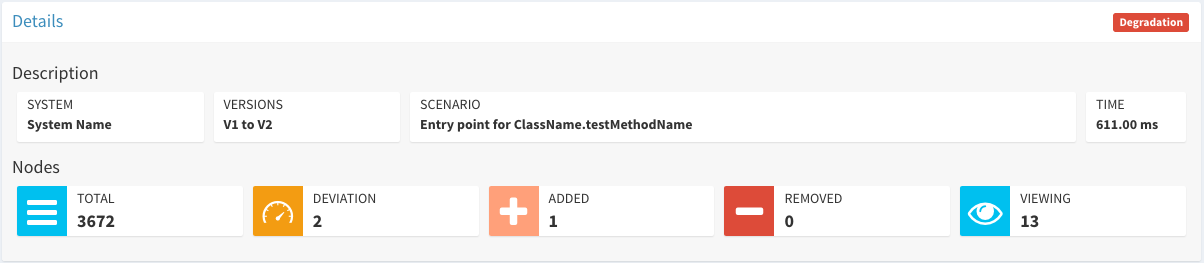
\includegraphics[scale=0.37]{Imagens/detalhes_grafo_chamadas.png}}
   \textsf{\caption[Seção de detalhes do grafo de chamadas.]{Seção de detalhes do grafo de chamadas.\label{fig:detalhes-grafo-chamadas}}}
\end{figure}

Na figura \ref{fig:detalhes-grafo-chamadas}, é mostrada uma visão geral sobre o cenário atual na visualização, contendo informações inerentes ao cenário. Para a seção \textit{Description}, as informações exibidas são:
\begin{itemize}
   \item \textit{System}: nome do sistema analisado;
   \item \textit{Versions}: versões do sistema que foram analisadas. É mostrado no formato \textit{<versionA>} to \textit{<versionB>}. Espera-se que a versão B, neste caso, seja posterior a versão A. No exemplo da figura, a versão V2 (\textit{versionB}) é posterior a versão V1 (\textit{versionA});
   \item \textit{Scenario}: exibe o nome do cenário analisado;
   \item \textit{Time}: mostra o tempo de execução do cenário na versão mais recente. A diferença de tempo entre as duas versões vai guiar o que será exibido na barra de títulos da figura. No exemplo mostrado, o tempo na última versão degradou com relação ao tempo na versão anterior, sendo exibido, no canto superior direito, um rótulo em vermelho marcando o cenário como degradado (\textit{degradation}). Caso o tempo do cenário seja otimizado, é exibido um rótulo verde marcando-o como otimizado (\textit{optimization}).
\end{itemize}

Para a seção \textit{Nodes}, as informações são as seguintes:
\begin{itemize}
   \item \textit{Total}: mostra o número total de nós do cenário. Vale salientar que cada nó representa um método executado durante a hierarquia de chamadas do cenário. Pode acontecer de nós diferentes representarem o mesmo método. Isso pode acontecer porque o mesmo método pode ser chamado hierarquias de chamadas diferentes;
   \item \textit{Deviation}: exibe o número de nós que tiveram algum desvio de desempenho. Para que um determinado nó seja considerado com desvio de desempenho, ele (i) tem que estar presente nas duas versões analisadas e (ii) tenha ocorrido diferenças, para mais ou para menos, no seu desempenho durante a execução do cenário nas versões analisadas;
   \item \textit{Added}: apresenta o número de nós que foram adicionados da versão anterior para a posterior. Ou seja, são os nós que não existiam na execução do cenário para a versão anterior e passaram a existir na execução da versão posterior;
   \item \textit{Removed}: o contrário do conceito anterior. São apresentados os nós que foram removidos da versão anterior para a posterior. Os nós removidos não são exibidos na visualização do grafo de chamadas;
   \item Viewing: apresenta a quantidade de nós que estão sendo mostrados no grafo de chamadas.
\end{itemize}

A segunda parte da visualização é o grafo de chamadas propriamente dito. Esse grafo, como mencionado, é composto de nós e arestas direcionadas que expõem os caminhos das chamadas dos métodos para o cenário analisado. Os nós, representados por caixas, possuem algumas características visuais, apresentadas adiante.

\begin{figure}[htb]
   \centering
   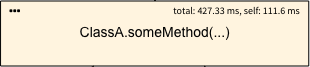
\includegraphics[scale=0.70]{Imagens/no_sem_desvio.png}
   \textsf{\caption[Nó que representa um método sem desvio de desempenho.]{Nó que representa um método sem desvio de desempenho.\label{fig:no-sem-desvio}}}
\end{figure}

O primeiro e mais básico tipo de nó é o que representa um método que não teve desvios de desempenho para o cenário e versões analisadas, apresentado na figura \ref{fig:no-sem-desvio}. As características desse nó são:\tabularnewline
\begin{itemize}
   \item \textit{Cor}: esta é a principal característica que diferencia os nós uns dos outros. No caso deste nó, a cor é marrom claro;
   \item \textit{Nome do nó}: posicionado ao centro, são mostrados o nome da classe e o nome do método executado, no formato \textit{ClassName.methodName()}. Para otimizar e evitar a exibição de grande quantidade de texto, o nome do pacote e os parâmetros do método foram ocultados, sendo estes representados por três pontos (...). Essa definição serve para todos os tipos de nós dessa visualização;
   \item \textit{Tempos de execução}: localizados no canto superior direito do nó, são apresentados dois tempos de execução: à esquerda, o tempo total do nó, que representa a soma dos tempos de execução dos nós filhos com o tempo do próprio nó. No exemplo da figura, o tempo total foi de 427,33 milissegundos; e à direita, o tempo do próprio nó, desconsiderando o tempo dos nós filhos. Na figura, o tempo foi de 111,6 milissegundos;
   \item \textit{Detalhes}: no canto superior esquerdo é exibido um ícone onde, ao passar o cursor do mouse, o usuário pode obter mais informações sobre o nó. No caso de um nó sem desvio de desempenho, as informações exibidas nesta seção são o nome do pacote e os parâmetros do método, se houver. A figura \ref{fig:detalhes-no-sem-desvio} a seguir mostra essa seção.
\end{itemize}

\begin{figure}[htb]
   \centering
   \frame{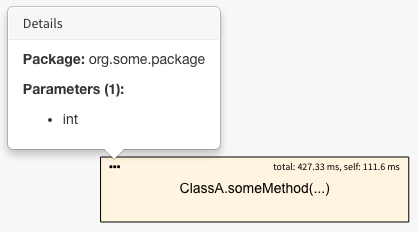
\includegraphics[scale=0.65]{Imagens/detalhes_no_sem_desvio.png}}
   \textsf{\caption[Seção de detalhes do nó sem desvio de desempenho.]{Seção de detalhes do nó sem desvio de desempenho.\label{fig:detalhes-no-sem-desvio}}}
\end{figure}

Quando um cenário possui nós que otimizaram o seu desempenho em relação à execução para a versão anterior, outros elementos visuais são acrescidos à visualização. A figura \ref{fig:no-otimizado} a seguir apresenta um nó otimizado:

\begin{figure}[htb]
   \centering
   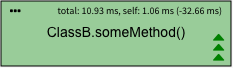
\includegraphics[scale=0.70]{Imagens/no_otimizado.png}
   \textsf{\caption[Nó que representa um método com otimização de desempenho.]{Nó que representa um método com otimização de desempenho.\label{fig:no-otimizado}}}
\end{figure}

As características visuais deste nó, além das comentadas anteriormente, são:
\begin{itemize}
   \item \textit{Cor}: os nós que otimizaram o atributo de qualidade desempenho são mostrados em um tom de verde;
   \item \textit{Tempos de execução}: além dos tempos total e do próprio nó, um nó com desvio de desempenho, seja otimização ou degradação, apresenta a diferença entre os tempos de execução da versão anterior para a posterior entre parênteses, no canto superior direito. No exemplo da figura, o nó melhorou o seu tempo em 32,66 milissegundos;
   \item \textit{Setas}: no canto inferior direito são mostradas setas indicativas de quão forte ou fraca foi a variação de desempenho. No caso de nós com otimização, são exibidas setas verdes apontadas para cima, onde cada uma delas representa 25\% de desvio do tempo com relação à versão anterior. Sendo assim, uma única seta representa um desvio de 0 a 25\%, duas setas de 25\% a 50\%, três setas de 50\% a 75\% e quatro setas de 75\% ou superior. No exemplo apresentado na figura \ref{fig:no-otimizado}, a otimização se deu entre 50\% e 75\% do desempenho anterior;
   \item \textit{Detalhes}: esta seção para os nós com otimização de desempenho possui informações diferentes das relatadas anteriormente, como podem ser vistas na figura \ref{fig:detalhes-no-otimizado}. Além das informações sobre o pacote e os parâmetros, também são apresentadas sobre os tempos de execução da versão anterior e posterior, além da variação de tempo.
\end{itemize}

\begin{figure}[htb]
   \centering
   \frame{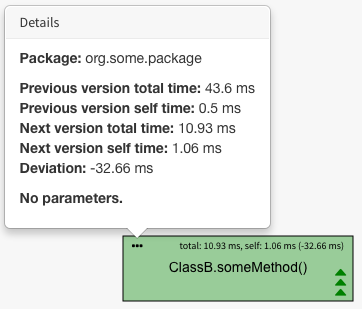
\includegraphics[scale=0.65]{Imagens/detalhes_no_otimizado.png}}
   \textsf{\caption[Seção de detalhes do nó com otimização de desempenho.]{Seção de detalhes do nó com otimização de desempenho.\label{fig:detalhes-no-otimizado}}}
\end{figure}

 A visualização também é capaz de apontar se determinado nó teve o seu desempenho degradado com relação à versão anterior. A figura \ref{fig:no-degradado} apresenta um nó degradado:

\begin{figure}[htb]
   \centering
   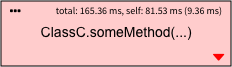
\includegraphics[scale=0.70]{Imagens/no_degradado.png}
   \textsf{\caption[Nó que representa um método com degradação de desempenho.]{Nó que representa um método com degradação de desempenho.\label{fig:no-degradado}}}
\end{figure}

As características visuais deste nó são bem semelhantes às apresentadas para os nós otimizados:
\begin{itemize}
   \item \textit{Cor}: os nós que degradaram o desempenho são mostrados em vermelho claro;
   \item \textit{Tempos de execução}: também são exibidos os tempos de execução total, do próprio nó e o desvio de desempenho. No exemplo, o nó degradou o tempo em 9,36 milissegundos;
   \item \textit: as setas indicativas de variação de desempenho para nós de degradação são apontadas para baixo, de cor vermelha. No exemplo, a degradação se deu entre 0 e 25\% do desempenho anterior;
   \item \textit{Detalhes}: esta seção possui as mesmas informações dos nós relatados até aqui, como podem ser vistas na figura \ref{fig:detalhes-no-degradado} a seguir.
\end{itemize}

\begin{figure}[htb]
   \centering
   \frame{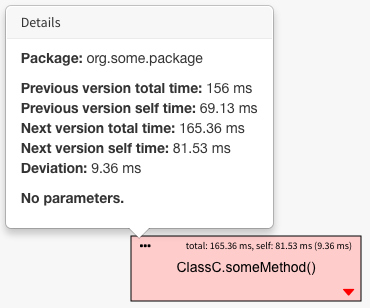
\includegraphics[scale=0.65]{Imagens/detalhes_no_degradado.png}}
   \textsf{\caption[Seção de detalhes do nó com degradação de desempenho.]{Seção de detalhes do nó com degradação de desempenho.\label{fig:detalhes-no-degradado}}}
\end{figure}

Um cenário pode apresentar, para diferentes versões, nós de chamadas de métodos que estão presentes na versão posterior, mas que não existiam na versão anterior. A visualização representa esses nós como mostra a figura \ref{fig:no-adicionado}. A descrição dos atributos visuais é a que segue:

\begin{figure}[htb]
   \centering
   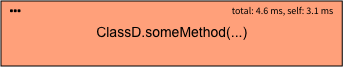
\includegraphics[scale=0.70]{Imagens/no_adicionado.png}
   \textsf{\caption[Nó que representa um método adicionado.]{Nó que representa um método adicionado.\label{fig:no-adicionado}}}
\end{figure}

\begin{itemize}
   \item \textit{Cor}: os nós que degradaram o desempenho são mostrados na cor salmão claro;
   \item \textit{Tempos de execução}: os tempos de execução total e do próprio nó são exibidos. No exemplo, o nó tem tempo total de em 4,6 milissegundos e o seu tempo é de 3,1 milissegundos.
   \item \textit{Detalhes}: nos nós adicionados, os detalhes possuem as mesmas informações exibidas para os nós de degradação ou de otimização. No entanto, uma mensagem é exibida em vermelho indicando que o nó adicionado é um potencial causador da degradação de desempenho do cenário. A figura \ref{fig:detalhes-no-adicionado} adiante apresenta esta seção.
\end{itemize}

\begin{figure}[htb]
   \centering
   \frame{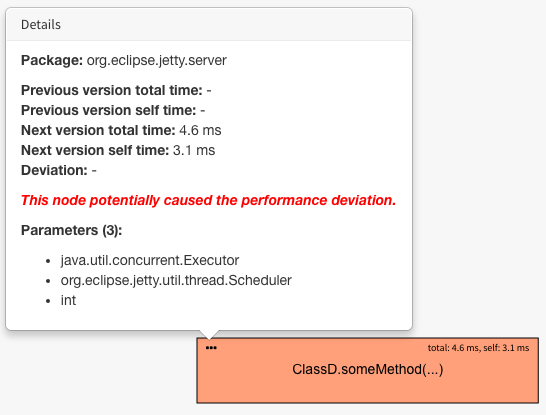
\includegraphics[scale=0.65]{Imagens/detalhes_no_adicionado.png}}
   \textsf{\caption[Seção de detalhes do nó adicionado.]{Seção de detalhes do nó adicionado.\label{fig:detalhes-no-adicionado}}}
\end{figure}

Além dos que representam métodos com ou sem desvio de desempenho, e métodos adicionados, há um tipo de nó que representa um agrupamento de vários outros: o agrupado. Assim, os que não estão diretamente relacionados com nós de desvio ou adicionados, são omitidos e representados por um único nó agrupado. A figura \ref{fig:no-agrupamento} a seguir ilustra esse tipo de nó, seguido da descrição dos seus atributos visuais.

\begin{figure}[htb]
   \centering
   \frame{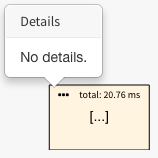
\includegraphics[scale=0.70]{Imagens/no_agrupamento.png}}
   \textsf{\caption[Nó que representa um agrupamento de outros nós.]{Nó que representa um agrupamento de outros nós.\label{fig:no-agrupamento}}}
\end{figure}

\begin{itemize}
   \item \textit{Cor}: os nós de agrupamento são mostrados na cor marrom claro;
   \item \textit{Nome do nó}: posicionado ao centro, é exibido o texto \textit{[...]};
   \item \textit{Tempos de execução}: é exibido o tempo de execução total que representa a soma de todos os tempos de execução dos nós contidos no agrupamento. No exemplo, o tempo total é de 20,76 milissegundos;
   \item \textit{Detalhes}: como pode ser percebido na imagem, este tipo de nó não possui detalhes a serem apresentados.
\end{itemize}

As propriedades visuais apresentadas para a visualização do grafo de chamadas incluem, em suma, duas partes: (i) seção de detalhes, contendo informações gerais sobre o cenário; e (ii) seção do grafo de chamadas, onde a execução dos métodos é representada através de nós e arestas. Esta seção é a mais importante desta visualização, contendo características visuais que diferem os nós de acordo com sua classificação. Um resumo dessas características é apresentado na tabela \ref{tab:resumo-caracteristicas-nos} a seguir.

\begin{table}[!htb]
   \textsf{\caption{Resumo das características visuais dos nós.\label{tab:resumo-caracteristicas-nos}}}
   \centering
   \medskip
   \begin{tabular}{c|c|c|c|c}
   \textbf{Tipo} & \textbf{Cor}   & \textbf{\begin{tabular}[c]{@{}c@{}}Tempos de\\ Execução\end{tabular}} & \textbf{Setas}                                                  & \textbf{Detalhes}                                                                     \\ \hline
   Sem desvio    & Marrom claro   & Total e próprio                                                       & Sem setas                                                       & \begin{tabular}[c]{@{}c@{}}Pacotes e \\ parâmetros\end{tabular}                       \\ \hline
   Degradado     & Vermelho claro & \begin{tabular}[c]{@{}c@{}}Total, próprio\\ e desvio\end{tabular}     & \begin{tabular}[c]{@{}c@{}}Vermelhas,\\ para baixo\end{tabular} & \begin{tabular}[c]{@{}c@{}}Pacotes, tempos\\ de execução e \\ parâmetros\end{tabular} \\ \hline
   Otimizado     & Verde claro    & \begin{tabular}[c]{@{}c@{}}Total, próprio\\ e desvio\end{tabular}     & \begin{tabular}[c]{@{}c@{}}Verdes,\\ para cima\end{tabular}     & \begin{tabular}[c]{@{}c@{}}Pacotes, tempos\\ de execução e \\ parâmetros\end{tabular} \\ \hline
   Adicionado    & Salmão claro   & Total e próprio                                                       & Sem setas                                                       & \begin{tabular}[c]{@{}c@{}}Pacotes, tempos\\ de execução e \\ parâmetros\end{tabular} \\ \hline
   Agrupado      & Marrom claro   & Total                                                                 & Sem setas                                                       & Sem detalhes
   \end{tabular}
\end{table}

\subsubsection{Interação} \label{subsec:interacao}

Esta visualização exibe um conjunto de informações que a torna capaz de indicar os métodos que potencialmente foram responsáveis por desvios de desempenho de um determinado cenário. Contudo, o usuário pode interagir com o grafo: (i) obtendo mais informações sobre um nó, passando o cursor do \textit{mouse} por cima do ícone de detalhes, como mostrado anteriormente; e (ii) executando o efeito de \textit{zoom} sobre o grafo para afastar ou aproximar a visualização. Esse efeito pode fazer com que o grafo seja comportado novamente na área de desenho.

\subsection{Funcionamento} \label{subsec:funcionamento-visualizacao-3}

A visualização utiliza os artefatos de saída gerados após a execução completa do \textit{PerfMiner}, de modo que se configura como mais uma etapa da ferramenta. A figura \ref{fig:perfminer-fase4} ilustra essa etapa. A extensão foi implementada em uma aplicação web, conforme explanado anteriormente e ilustrado na figura \ref{fig:funcionamento-geral-visualizacoes}. Embora o funcionamento mostrado nessa figura seja geral, são necessários processamentos específicos para esta visualização, a fim de tratar os dados para serem exibidos para o usuário.

Para esta visualização, seguindo o funcionamento mostrado na figura \ref{fig:funcionamento-geral-visualizacoes}, o usuário realiza a requisição para esta visualização, passando como parâmetros o nome do sistema e as duas versões (passo 1). Os passos 2 e 3, em detalhes, é exibido na figura \ref{fig:passos-2-3-grafo-chamadas}.

\begin{figure}[!htb]
   \centering
   \frame{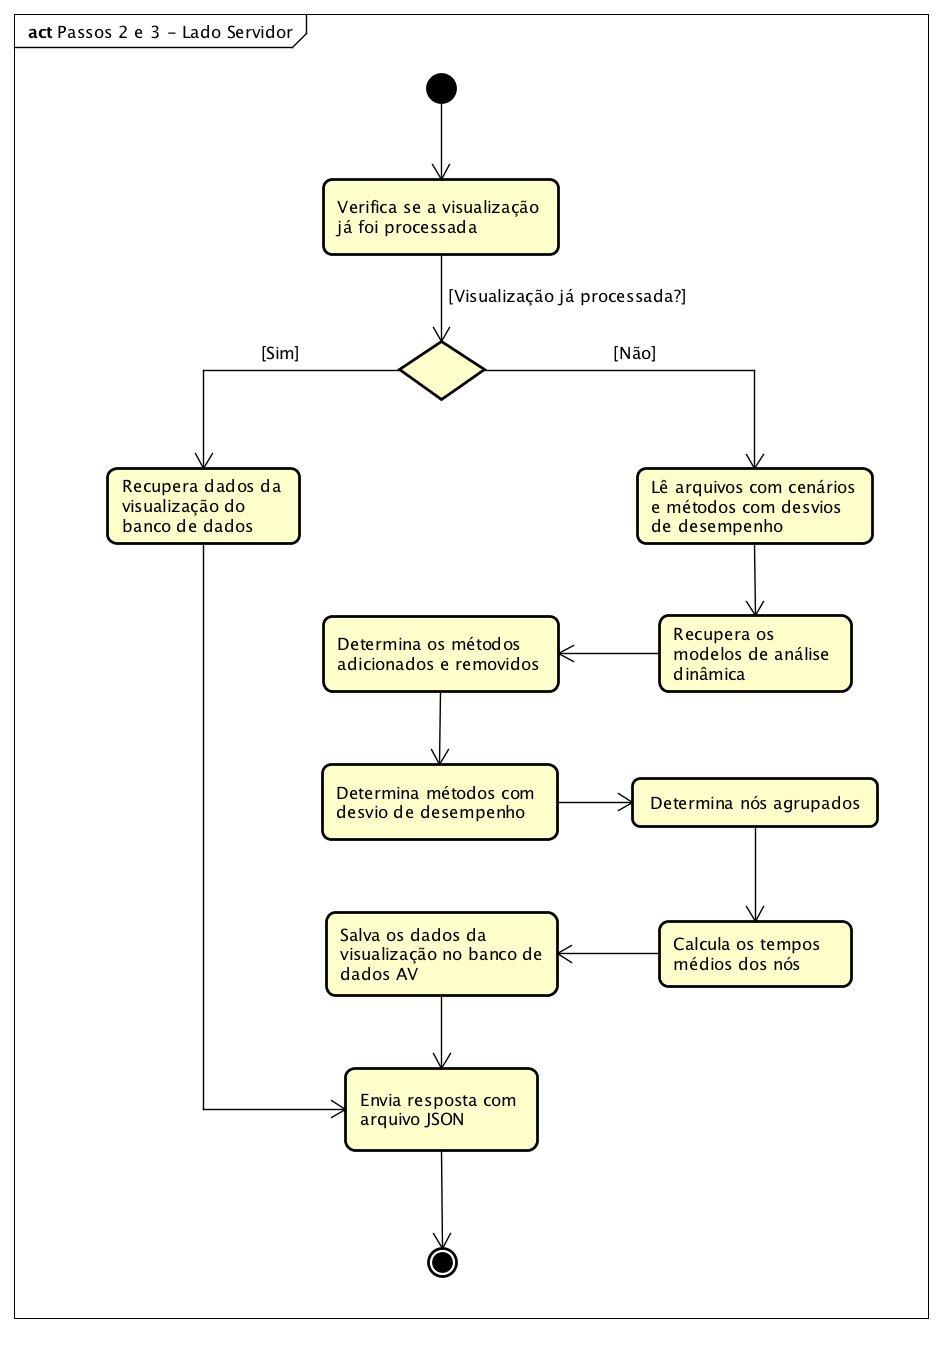
\includegraphics[scale=0.45]{Imagens/visualizacao_3_fase_2_e_3.png}}
   \textsf{\caption[Passos 2 e 3 da visualização grafo de chamadas.]{Passos 2 e 3 da visualização grafo de chamadas.\label{fig:passos-2-3-grafo-chamadas}}}
\end{figure}

O processo se inicia quando o servidor recebe a requisição do usuário, solicitando a visualização do grafo de chamadas para determinadas versões de um sistema. Ao receber, a aplicação verifica se a visualização requerida já foi processada anteriormente, consultando-a no banco de dados QAV. Em caso positivo, os dados são recuperados, o arquivo JSON é montado e enviado na resposta do servidor, e o processo acaba.

Caso a visualização ainda não tenha sido processada, os arquivos de saída do \textit{PerfMiner} contendo informações sobre os cenários e métodos com desvio de desempenho são lidos e os modelos de análise dinâmica de ambas as versões são recuperados do banco de dados DAM. Esse modelo é formado por um grafo com todos os nós de chamadas dinâmico que representa cada execução do cenário.

De posse dos nós recuperados, são determinados os métodos que foram adicionados ou removidos comparando os nós da versão atual com os da anterior. Depois disso, a partir dos métodos indicados pelos arquivos de saída do \textit{PerfMiner}, são determinados os nós com desvios de desempenho, seja degradação ou otimização.

Na extensão, os nós identificados como adicionados e com desvio são candidatos a serem exibidos. Optou-se por apresentar apenas os nós com desvio, nós adicionados e alguns nós sem desvio de desempenho, mas que garantem o entendimento do grafo, de modo que poucos nós são renderizados no navegador do usuário. Essa decisão levou em consideração a quantidade de nós de um cenário, que facilmente pode passar dos milhares, o desempenho da própria aplicação web e a eficácia no entendimento da visualização por parte do usuário. Espera-se que, com menos nós exibidos, os usuários consigam entender e acompanhar mais claramente a evolução do atributo de qualidade de desempenho.

Após determinar os nós com desvios de desempenho, são criados nós de agrupamento para representar os nós que não serão exibidos na visualização. Depois disso, os tempos médios dos nós a serem exibidos são calculados, levando em consideração todas as ocorrências do método no cenário. Após, os dados do processamento são salvos no banco de dados QAV e, por fim, o arquivo JSON que dá suporte à visualização é montado e enviado como resposta do servidor, e o processo acaba.

Quando o usuário recebe a resposta, há um procedimento executado no seu navegador, que recebe e processa o arquivo JSON e, ao final, renderiza o grafo de chamadas. Esse processo representa o passo 5 da figura \ref{fig:funcionamento-geral-visualizacoes} está exposto em detalhes na figura \ref{fig:passo-5-grafo-chamadas} adiante. O início ocorre ao receber o arquivo do servidor e a primeira atividade é criar a área de desenho que abrigará o grafo. Nessa atividade são considerados a altura e largura do monitor do usuário, de modo que a área útil de apresentação seja compatível com a área do monitor.

\begin{figure}[!htb]
   \centering
   \frame{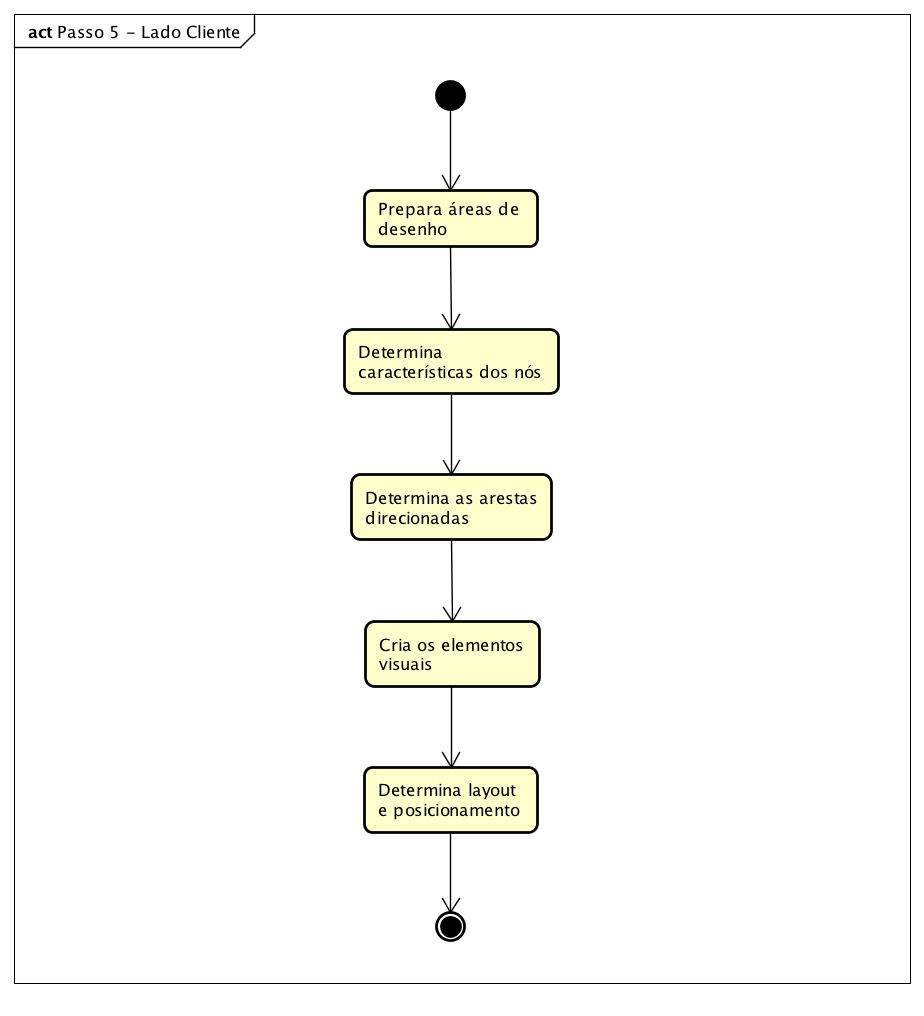
\includegraphics[scale=0.50]{Imagens/visualizacao_3_fase_5.png}}
   \textsf{\caption[Passos 5 da visualização grafo de chamadas.]{Passos 5 da visualização grafo de chamadas.\label{fig:passo-5-grafo-chamadas}}}
\end{figure}

Após isso, as características dos nós contidos no arquivo JSON são determinadas. Para cada um deles, são determinados: (i) a altura e largura da sua caixa, que é diretamente proporcional ao tamanho do nome a ser exibido. Vale salientar que o pacote da classe é omitido para a exibição do nome; (ii) a cor, que depende do seu tipo; (iii) os tempos de execução total e, caso pertinente, o do próprio nó e o de desvio; (iv) as setas, que dependem do seu tipo e da porcentagem de desvio do tempo de execução ocorrida de uma versão para outra; e (v) os detalhes, que dependem do tipo do nó.

Depois, as arestas são determinadas de acordo com a relação de nós pais e filhos contidos no arquivo. Elas são direcionadas do nó pai para os filhos, indicando a hierarquia de chamadas.

Com a definição dos nós e suas características, e das arestas, a próxima atividade do processo é criar os elementos visuais na área de desenho, para, posteriormente, determinar o \textit{layout} (conforme citado anteriormente, o \textit{layout} utilizado é em árvore) e posicionamento dos nós. Por fim, o grafo de chamadas é renderizado para o usuário.

\subsection{Exemplo de Uso da Ferramenta: Jetty} \label{subsec:exemplo-uso-jetty}

Foi realizado um estudo de caso para exemplificar o uso das visualizações. Para tanto, foi utilizado duas versões da aplicação Jetty \cite{Jetty2016}: 9.2.6 e 9.3.0.M1. Esse sistema faz parte do Projeto Eclipse e é um \textit{framework open-source} que provê um servidor web além de um servlet container Java. Essa aplicação foi escolhida para o estudo de caso pois todos os tipos de nós foram capazes de ser exemplificados.

Para a primeira fase do \textit{PerfMiner}, a análise dinâmica, todos os testes automatizados foram considerados cenários. Como os testes são implementados em JUnit 4, o aspecto interceptou todos os métodos marcados com a anotação \texttt{@Test} como métodos de entrada de um cenário. A análise dinâmica, como mencionado anteriormente, foi executada no mesmo computador para ambas as versões, nas mesmas condições e com todos os serviços não essenciais desabilitados. A suíte de testes do Jetty foi executada 30 vezes para que as medições de desempenho fossem mais precisas em termos de tempo de execução \cite{Pinto2015}.

A resultado da análise foi um total de 11 cenários, sendo 7 com degradação do desempenho e 4 com otimização. No grafo gerado, é possível que dois nós representem o mesmo método, indicando duas execuções, e as arestas direcionadas representam invocações entre os métodos. A figura \ref{fig:exemplo-degradacao} exemplifica o grafo de um cenário com degradação.

\begin{figure}[!htb]
   \centering
   \frame{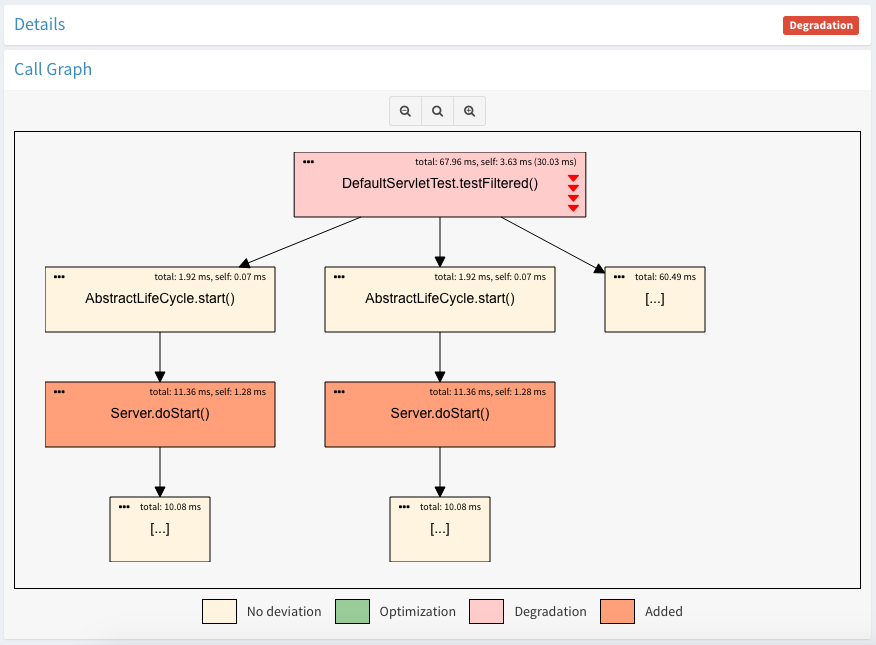
\includegraphics[scale=0.52]{Imagens/exemplo_degradacao.png}}
   \textsf{\caption[Grafo de chamadas de um cenário com degradação de desempenho.]{Grafo de chamadas de um cenário com degradação de desempenho.\label{fig:exemplo-degradacao}}}
\end{figure}

O grafo exibido destaca que o nó raiz, \texttt{DefaultServletTest.testFiltered()}, teve uma degradação de desempenho de mais de 75\%, indicado pela cor do nó, vermelho claro, e pelas quatro setas vermelhas para baixo. É possível notar também que dois nós que representam o método \texttt{Server.doStart()} foram adicionados. Isso significa que durante a execução do cenário \texttt{Entry point for DefaultServletTest.testFiltered} duas chamadas a esse método foram efetuadas na versão 9.3.0.M1, e elas não existiam na versão 9.3.6. Os nós adicionados são indicados como potenciais causadores de degradação de desempenho, de modo que, possivelmente, esses nós influenciaram na degradação do raiz. Na visualização há nós que não têm relação com os desvios, representados como agrupados, e nós sem desvio, representados na cor marrom claro.

Na mesma figura, além do próprio grafo, na parte superior da seção \textit{Call Graph} é encontrada uma barra de ferramentas com botões de \textit{Zoom Out}, \textit{Zoom to Fit} e \textit{Zoom In}; e na parte inferior é exibida uma legenda ajudando os usuários a identificarem os nós do grafo. Os botões de \textit{zoom} e a legenda são exibidos para todos os grafos, independente da quantidade de nós ou do tipo de desvio ocorrido.

Na figura \ref{fig:exemplo-detalhes-degradacao} adiante, a seção \textit{Details} desse cenário é exibida expandida, indicando, no rótulo, que o cenário teve o seu desempenho degradado entre as versões, e que o total de nós para esse cenário foi de 1695.

\begin{figure}[!htb]
   \centering
   \frame{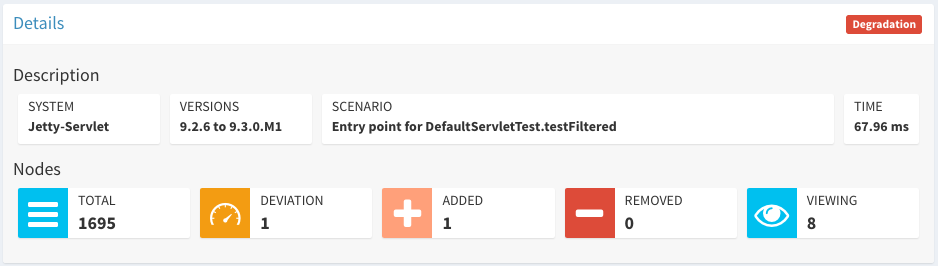
\includegraphics[scale=0.48]{Imagens/exemplo_detalhes_degradacao.png}}
   \textsf{\caption[Detalhes de um cenário com degradação de desempenho.]{Detalhes de um cenário com degradação de desempenho.\label{fig:exemplo-detalhes-degradacao}}}
\end{figure}

A figura \ref{fig:exemplo-otimizacao} a seguir apresenta o cenário \texttt{Entry point for ServletContextHandler\\Test.testFallThrough} com otimização de desempenho. Dois nós contribuíram para esse desvio, identificados pela cor verde claro: \texttt{Server.doStart()} e \texttt{ServletContextHandler.\\relinkHandlers()}. No primeiro, a variação foi entre 50\% e 75\%, ao passo que no segundo foi de mais de 75\%. Há ainda a representação de nós agrupados e sem desvio.

\begin{figure}[!htb]
   \centering
   \frame{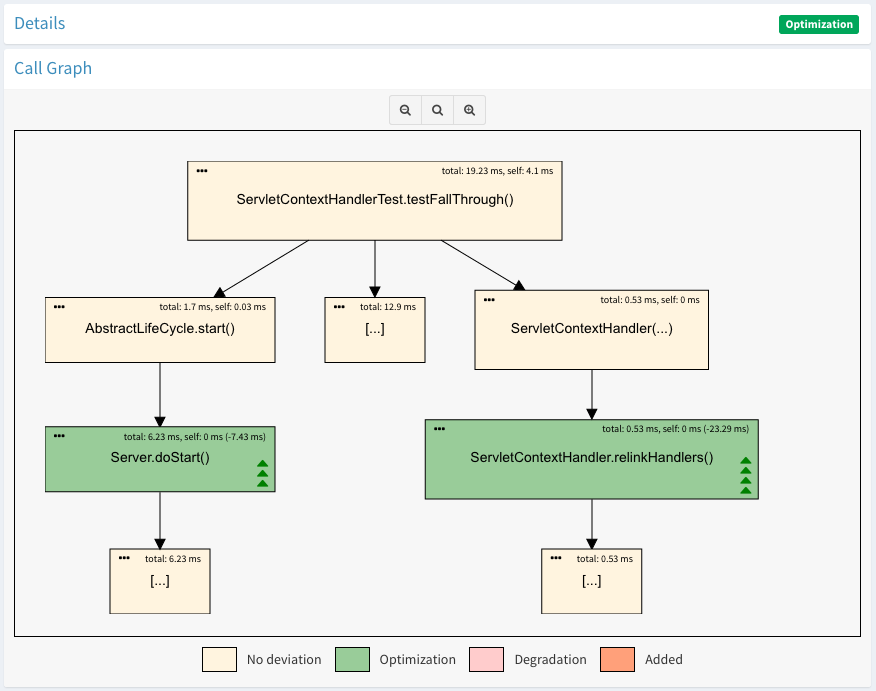
\includegraphics[scale=0.52]{Imagens/exemplo_otimizacao.png}}
   \textsf{\caption[Grafo de chamadas de um cenário com otimização de desempenho.]{Grafo de chamadas de um cenário com otimização de desempenho.\label{fig:exemplo-otimizacao}}}
\end{figure}

\begin{figure}[!htb]
   \centering
   \frame{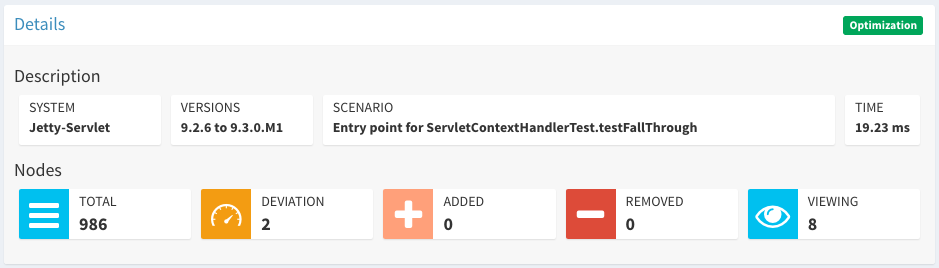
\includegraphics[scale=0.48]{Imagens/exemplo_detalhes_otimizacao.png}}
   \textsf{\caption[Detalhes de um cenário com otimização de desempenho.]{Detalhes de um cenário com otimização de desempenho.\label{fig:exemplo-detalhes-otimizacao}}}
\end{figure}

A seção \textit{Details} expandida pode ser vista na figura \ref{fig:exemplo-detalhes-otimizacao}. O rótulo de otimização é exibido no canto superior esquerdo indicando o tipo de desvio ocorrido no cenário. A figura indica um total de 986 nós para esse cenário.

A tabela \ref{tab:jetty-v9.2.6-v9.3.0.M1} a seguir mostra uma lista com todos os cenários para o sistema Jetty, versões 9.2.6 para 9.3.0.M1. Nela, são exibidas as porcentagens de desvio de degradação ou otimização para os cenários.

\begin{sidewaystable}[!htb]
   \textsf{\caption{Cenários para o Jetty, versões 9.2.6 para 9.3.0.M1.\label{tab:jetty-v9.2.6-v9.3.0.M1}}}
   \centering
   \medskip
   \begin{tabular}{l|c|c|c|c}
   \multicolumn{1}{c|}{\textbf{Nome}}                                                                                                       & \textbf{\begin{tabular}[c]{@{}c@{}}Tempo \\ v9.2.6 (ms)\end{tabular}} & \textbf{\begin{tabular}[c]{@{}c@{}}Tempo \\ v9.3.0.M1 (ms)\end{tabular}} & \textbf{\begin{tabular}[c]{@{}c@{}}Variação \\ (\%)\end{tabular}} & \textbf{\begin{tabular}[c]{@{}c@{}}Tipo de \\ Desvio\end{tabular}} \\ \hline
   \begin{tabular}[c]{@{}l@{}}Entry point for \\ DispatcherForwardTest.testQueryRetainedByForward\\ WithoutQuery\end{tabular}              & 569,26                                                                & 597,33                                                                   & 4,93                                                              & Degradação                                                         \\ \hline
   \begin{tabular}[c]{@{}l@{}}Entry point for \\ SSLAsyncIOServletTest.testAsyncIOWritesWith\\ Aggregation\end{tabular}                    & 549,21                                                                & 587,55                                                                   & 6,98                                                              & Degradação                                                         \\ \hline
   \begin{tabular}[c]{@{}l@{}}Entry point for \\ AsyncServletLongPollTest.testSuspendedRequest\\ CompletedByAnotherRequest\end{tabular}    & 620,36                                                                & 634,60                                                                   & 2,29                                                              & Degradação                                                         \\ \hline
   Entry point for DefaultServletTest.testFiltered                                                                                         & 37,93                                                                 & 67,96                                                                    & 79,17                                                             & Degradação                                                         \\ \hline
   \begin{tabular}[c]{@{}l@{}}Entry point for \\ ServletContextHandlerTest.testReplaceServlet\\ HandlerWithoutServlet\end{tabular}         & 429,60                                                                & 453,96                                                                   & 5,67                                                              & Degradação                                                         \\ \hline
   \begin{tabular}[c]{@{}l@{}}Entry point for \\ AsyncContextListenersTest.testAsyncDispatch\\ AsyncCompletePreservesListener\end{tabular} & 601,83                                                                & 622,96                                                                   & 3,51                                                              & Degradação                                                         \\ \hline
   \begin{tabular}[c]{@{}l@{}}Entry point for \\ AsyncIOServletTest.testAsyncWriteThrowsError\end{tabular}                                 & 599,10                                                                & 611,00                                                                   & 1,98                                                              & Degradação                                                         \\ \hline
   \begin{tabular}[c]{@{}l@{}}Entry point for \\ DispatcherForwardTest.testQueryAggregatesWith\\ FormByForwardWithoutQuery\end{tabular}    & 26,46                                                                 & 20,76                                                                    & 21,54                                                             & Otimização                                                         \\ \hline
   \begin{tabular}[c]{@{}l@{}}Entry point for \\ ServletContextHandlerTest.testFallThrough\end{tabular}                                    & 52,00                                                                 & 19,23                                                                    & 63,01                                                             & Otimização                                                         \\ \hline
   \begin{tabular}[c]{@{}l@{}}Entry point for \\ AsyncContextListenersTest.testListenerCleared\\ OnSecondRequest\end{tabular}              & 23,90                                                                 & 17,16                                                                    & 28,20                                                             & Otimização                                                         \\ \hline
   \begin{tabular}[c]{@{}l@{}}Entry point for \\ ServletContextHandlerTest.testAddServletAfterStart\end{tabular}                           & 55,56                                                                 & 20,40                                                                    & 63,28                                                             & Otimização                                                     
   \end{tabular}
\end{sidewaystable}

A maior variação absoluta foi para o cenário \texttt{Entry point for DefaultServletTest\\.testFiltered}, uma degradação de 79,17\%. Como destacado na figura \ref{fig:exemplo-degradacao}, dois nós com tempos significantes com relação ao cenário foram adicionados, provavelmente, causando a degradação. O gráfico \ref{fig:grafico-jetty-v9.2.6-v9.3.0.M1} adiante exibe a porcentagem de variação de desempenho.

\begin{sidewaysfigure}[!htb]
   \centering
   \frame{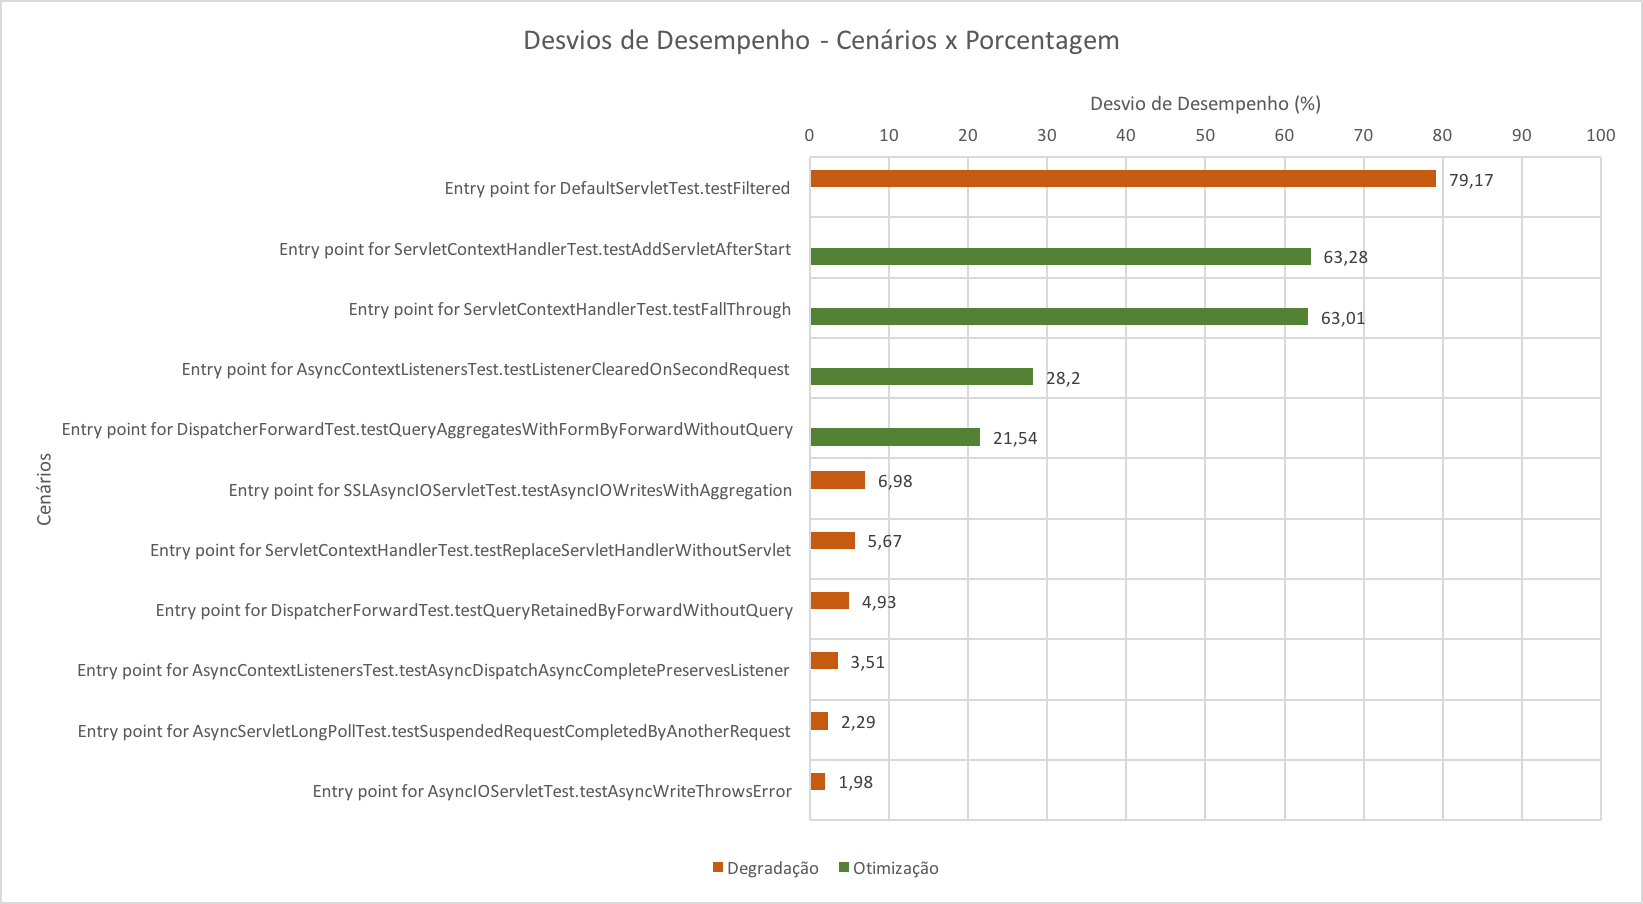
\includegraphics[scale=0.80]{Imagens/grafico_jetty_v926_v931M1.png}}
   \textsf{\caption[Porcentagem de desvios de desempenho para o Jetty, versões 9.2.6 para 9.3.0.M1.]{Porcentagem de desvios de desempenho para o Jetty, versões 9.2.6 para 9.3.0.M1.\label{fig:grafico-jetty-v9.2.6-v9.3.0.M1}}}
\end{sidewaysfigure}

\section{Considerações} \label{sec:consideracoes-cap3}


Um dos principais desafios do processo de manutenção de um software é compreendê-lo adequadamente, em especial, a sua arquitetura. A falta de acompanhamento da evolução da arquitetura ao longo do tempo pode levar a sua degradação, impactando os seus atributos de qualidade. Este capítulo apresentou visualizações de arquitetura de software que visam tornar direta e fácil a monitoração da evolução arquitetural, com relação ao atributo de qualidade de desempenho. Uma vez que as ferramentas existentes se mostram complexas ou ineficientes para essa finalidade, as visualizações foram propostas a serem implementadas como extensões da ferramenta \textit{PerfMiner}. Em suma, são as seguintes:
\begin{enumerate}[(i)]
   \item \textit{Evolução do Desempenho}: a evolução do atributo de qualidade de desempenho pode ser acompanhada em outra visualização, que mostra, para cada versão do sistema, se este degradou, otimizou ou manteve estável o seu desempenho;
   \item \textit{Sumarização dos Cenários}: a sumarização dos cenários com desvio de desempenho objetiva mostrar, de maneira sucinta, quais cenários analisados tiveram desvio de desempenho, seja degradação ou otimização;
   \item \textit{Grafo de Chamadas}: a visualização do grafo de chamadas exibe, para cada cenário, as chamadas dos métodos que tiveram desvio de desempenho. Dessa forma, o usuário pode localizar em qual trecho de código da execução do cenário houve o desvio.
\end{enumerate}

Foi mostrado os detalhes da visualização do grafo de chamadas, que visa exibir, para dadas duas versões de um sistema, os métodos que potencialmente causaram o desvio de desempenho para um determinado cenário. Nesta visualização, os métodos são apresentados em um grafo direcionado de chamadas com propriedades visuais que destacam quais dos métodos mostrados tiveram desvios de desempenho.

É importante frisar que a implementação das visualizações ainda não está finalizada. As duas primeiras mencionadas neste capítulo, evolução do desempenho e sumarização dos cenários, ainda estão em fase de concepção, ao passo que a terceira, grafo de chamadas, está em fase de conclusão. Para esta última, ainda serão adicionados, na seção de detalhes dos nós, \textit{links} para os \textit{commits} e tarefas que alteraram o método representado. Para cada método com desvio, serão recuperados os \textit{commits} do sistema de controle de versões e verificado quais commits alteraram linhas dentro do método detectado. Para cada um dos que alteraram, o número da respectiva tarefa é procurado na mensagem de \textit{commit}. Este número é usado para procurar a tarefa no sistema de gerenciamento de tarefas em busca de informações extras, como o seu tipo.

\section{Ameaças à validade} \label{sec:ameacas}